\documentclass{beamer}

\usetheme{PaloAlto}

\usepackage{graphicx} % Required for inserting images
\usepackage{amsmath,amssymb}

\DeclareMathOperator{\E}{\mathbb{E}}

\title{The Impact of Imputation Quality \\ on Family Based Analysis}
\author[]{Mahdi Mir}
\date[]{May 2024}

\begin{document}

\maketitle


\begin{frame}[label=outl]
    \frametitle{Outline}
    \tableofcontents{}
\end{frame}


\section{Introduction}


\begin{frame}{Introduction}


\begin{itemize}
      \item We are concerned that low quality imputed genotypes may not work for family based analysis.
      % not all imputed genotypes are bad its more lower quality imputed genotypes might be bad.
      \item E.g.: Howe et.al (2022) Sib-GWAS paper used low quality imputed SNPs in its analysis. % Than may be an issue.
      \item They use hard-calls data for SNPs with info score \(> 0.3\).
      \item Initially, I was focused only on the imputed data. I exteneded one of the Tammy's analysis to the whole genome.
\end{itemize}

    
\end{frame}


\begin{frame}{Background}
      
% I'll give more background to make you more interested to make it clear why it is important and why it is interesting

\begin{itemize}
      % so there are these family based designs that we are intereseted in and 
      % other people are interested in such as gwas or controlling for parental genotypes
      % and they rely on some specific family based data properties that are not might be preserved 
      % in low qulity imputed snps 
      
      \item There are these family-based research desings like what we have in the within-family
      project that rely on special properties of family data. % like the random assignment of genotypes within family 
      \item E.g.: random assignment of genotypes within families.
      
      % one of the designs that Howe et al used is sib-gwas
      \item Howe et.al. (2022) used the genetic differences between sibs.
      % we are concerned that doing that, using genetic differences between sibs when using 
      % low quality imputed SNPs. It doesn't have the right properties for those estimates to be uncounfounded or 
      % using them to make causal inferences.
      % so people are using the quality imputed SNPs that 
\end{itemize}


\end{frame}


\begin{frame}{Motivation}
      
      \begin{itemize}
            \item Based on the Mandellian laws we expect that the correlation between parent-offspring and sibling pairs to be 0.5.
            \item One way to detect issues in the imputed data is that if the correlation between sibling pairs and parent-offspring pairs deviates from 0.5.
            \item Assume \(i\) and \(j\) to be either siblings pairs or parent-offspring pairs, then theoretically we have:
      \end{itemize}

      \[
            Corr(G_i, G_j) = 0.5
      \]

      \begin{itemize}
            \item But the question is: % do we have it in the imputed data that are an estimation of the real data
      \end{itemize}

      \[
            Corr(\hat{G_i}, \hat{G_j}) \; =? \; 0.5    
      \]

\end{frame}



\section{Correlation Analysis}



\begin{frame}{Correlation Analysis on the Imputed Data}
    

      \begin{itemize}
          \item In theory, we should see 0.5 correlation between both full-sibling and parent-offspring pairs genotypes.
          \item So if the imputed genotypes is high quality imputed then we should see the distribution of correlations to be concentrated around the half.
          \item Expectation: we would expect more deviation for low quality SNPs from the theoretical expectation.
      \end{itemize}
      

\end{frame}

% in this part we have some nice figures to show to you that conveys the whole point we are going to show.
% there are some really minute and small steps that I took that I didn't mention them here because it gets too technical but just 
% to say each of these steps as you know when you are writng and testing and developing the code every step could be 
% Challening, but addressing each of them would be too much technical talk.

% mention the repos that I created so far


\begin{frame}{Sample}
    
\begin{itemize}

      \item UKB Imputed Data.
      \item We have a sample of \(\backsimeq 20,000\) of sibling pairs. % I guess this is the full sample of full-sbiling pairs in the UKB data.
      \item \(\backsimeq 4000\) parent-offspring pairs.
      \item For each info score we selected 1000 SNPs randomly from the enitre genome.

\end{itemize}

\end{frame}



\begin{frame}{What is Info Score?}

      \begin{itemize}
            \item For each imputed SNP we have an info score between zero and one which gives us the quality of imputation.
            \item If it is closer to 1 the higher the quality of imputation is and the more we are confident that the imputation is close to reality. 
            \item And the more it is closer to 0 we are less confident that is true.
      \end{itemize}

      \[ \forall \text{ Imputed SNP } : 0 < \text{Info Score} < 1\]

\end{frame}



\begin{frame}{Dosages vs. Hard-Calls Genotypes}

      \begin{itemize}
            \item Imputation methods gives us for each SNP a discrete probablity distribution on 3 points.
            % the third one would be determined when we know the first two because like any other probability disribution the sum is 1.
            \item If we get the expectation of those probabilities we call it dosages. % so we have the probaliblity of the genotype at some SNP to be zero 
            % and we have the probability of it to be 1 and to be 2 if we get the expecation we have dosages:
      \end{itemize}

      \[
           \text{Dosages} = \E(\hat{G}) = 0\times P[G=0] + 1\times P[G=1] + 2 \times P[G=2]  
           % writing the 0 times p(0) doesn't make much sense but I wanted to be more clear    
      \]

      \begin{itemize}
            \item If we just pick the most probable genotype then we have the hard-call for the SNP.
      \end{itemize}

      \[
            \text{Hard-Call} = \operatorname*{argmax}_{G \in \{0,1,2\}} P(G)
      \]

\end{frame}


% lets see some plots 
% zoom in this slide during the presentation
% there are some things in these graphs that we don't have description for it yet.

\begin{frame}{Correlations Distribution}{High Quality SNPs - Full Siblings - Dosages}

      \centering     
      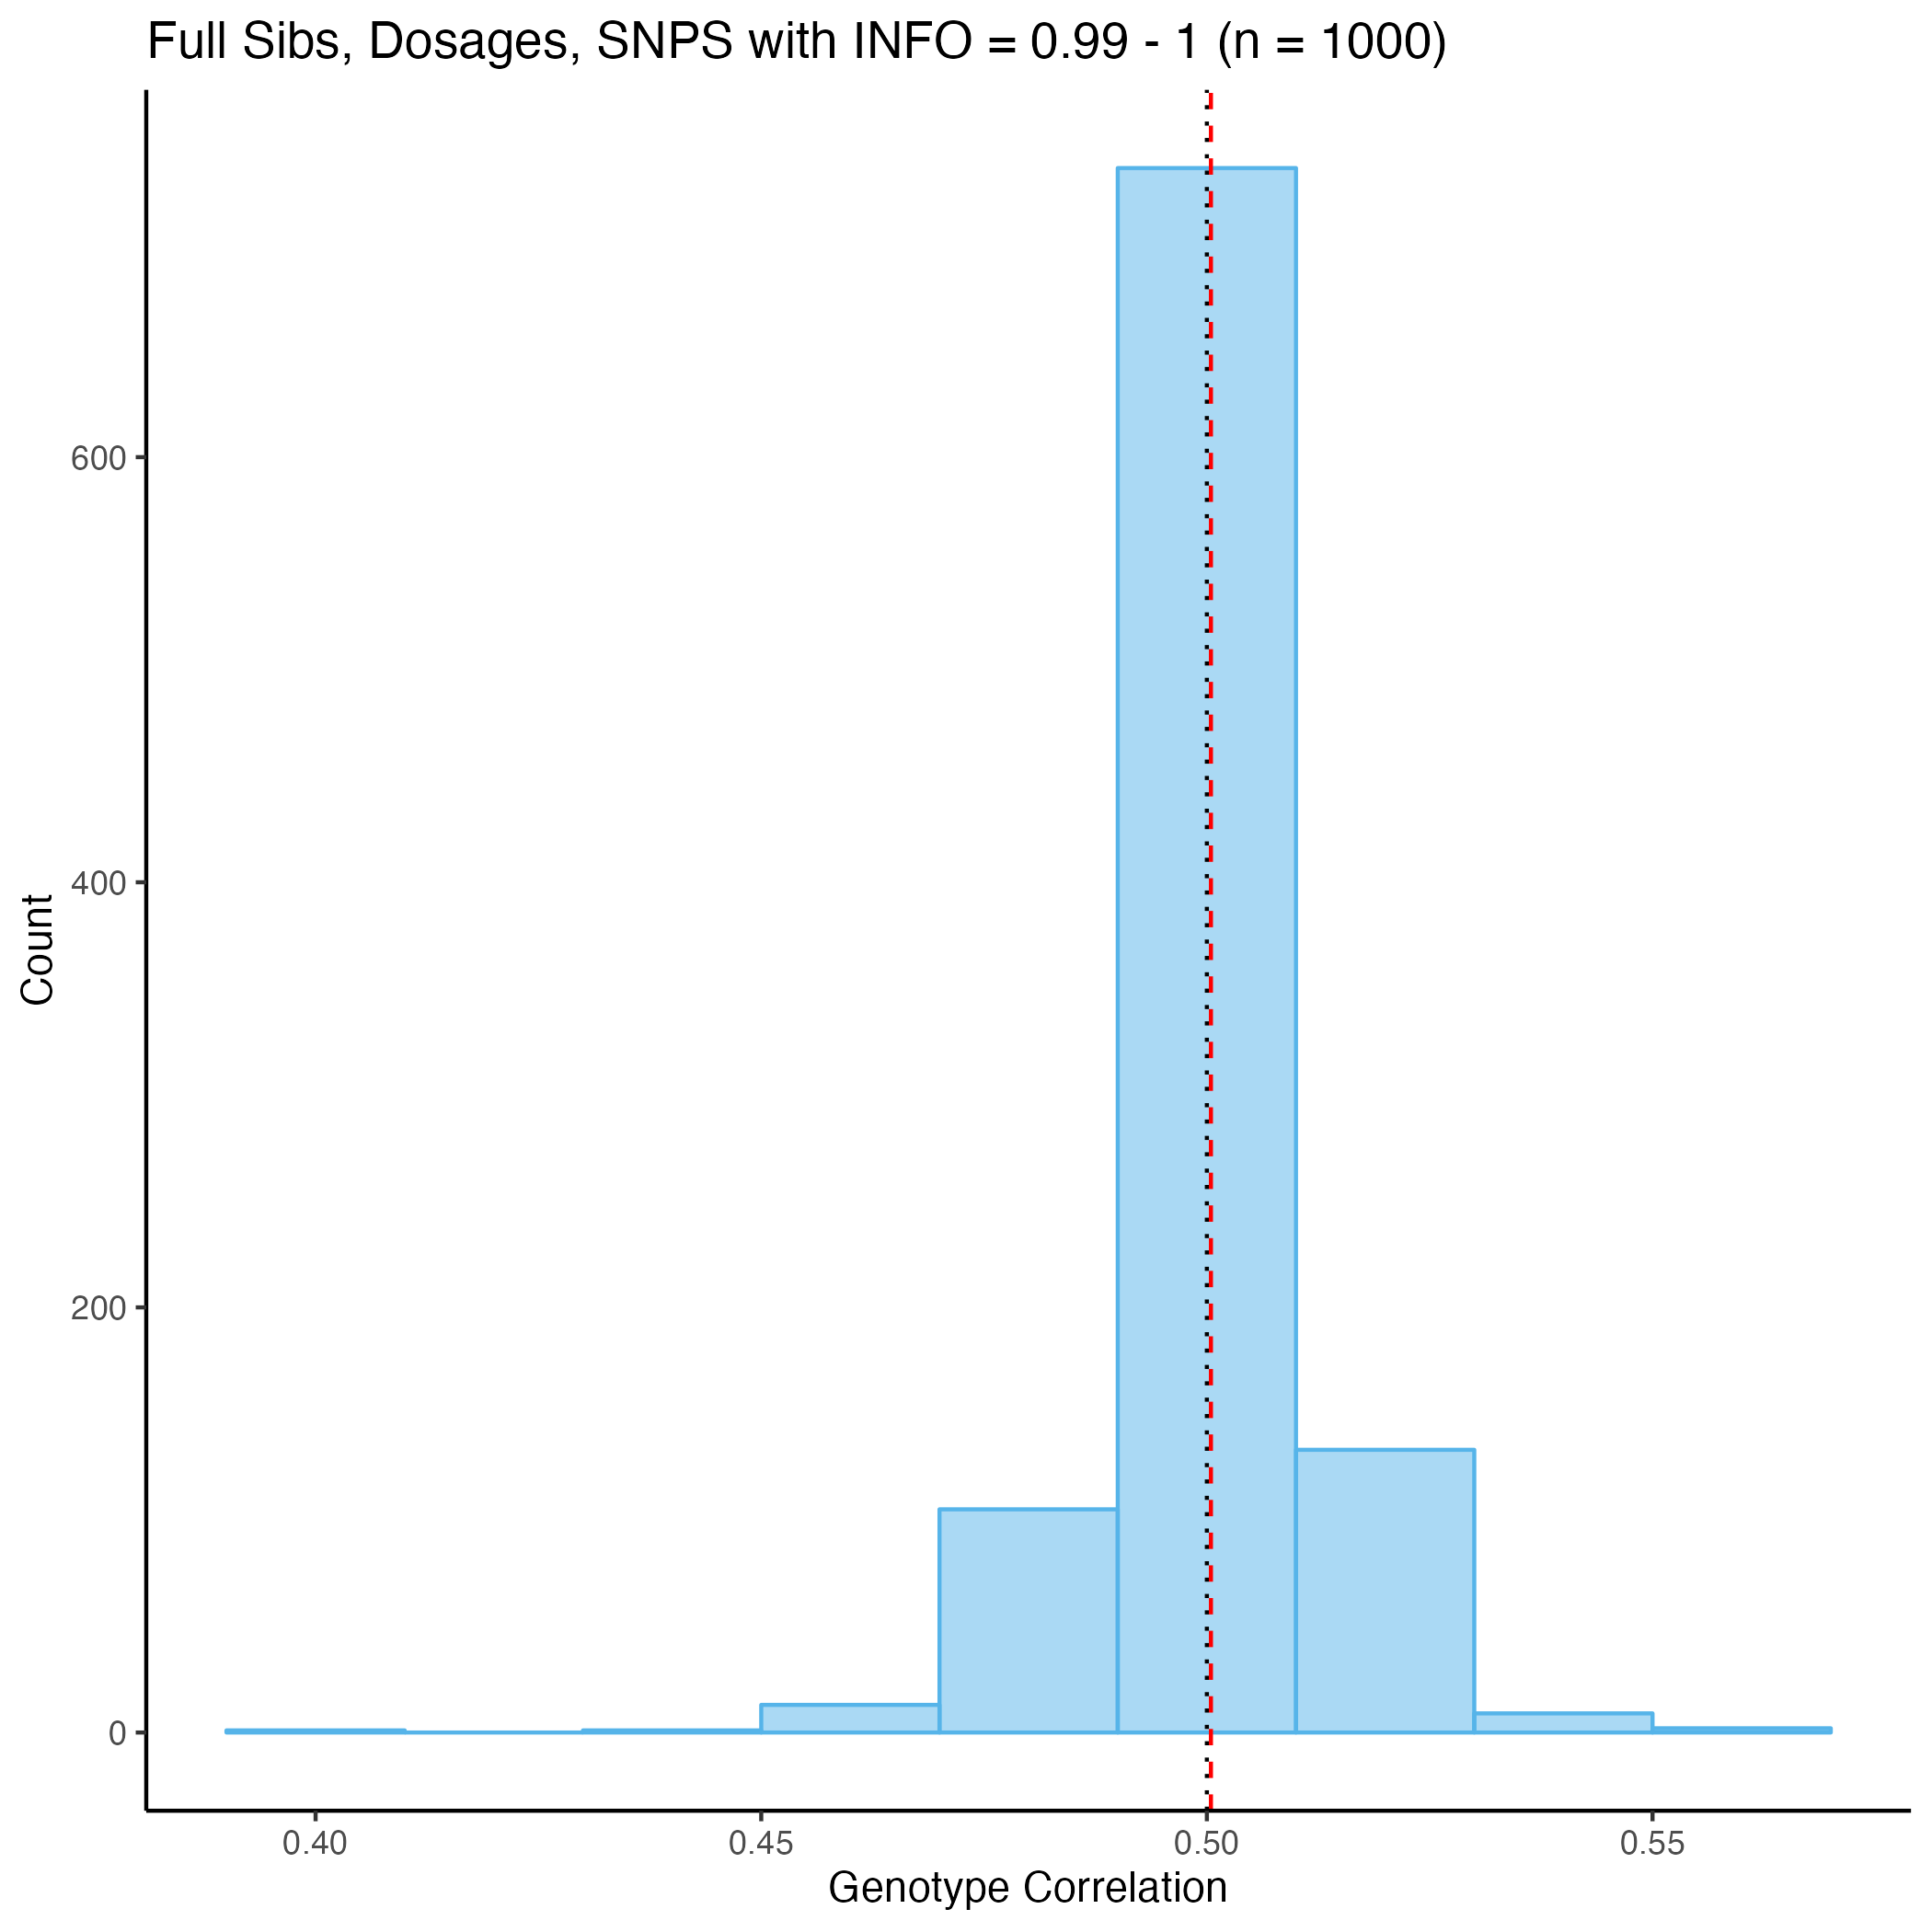
\includegraphics[width= .7\textwidth]{fig/FS-DSG-i99.png}
      % As you can see with high quality SNPs it gives the expected results according to theory

\end{frame}


\begin{frame}{Correlations Distribution}{High Quality SNPs - Full Siblings - Hard Calls}

      \centering     
      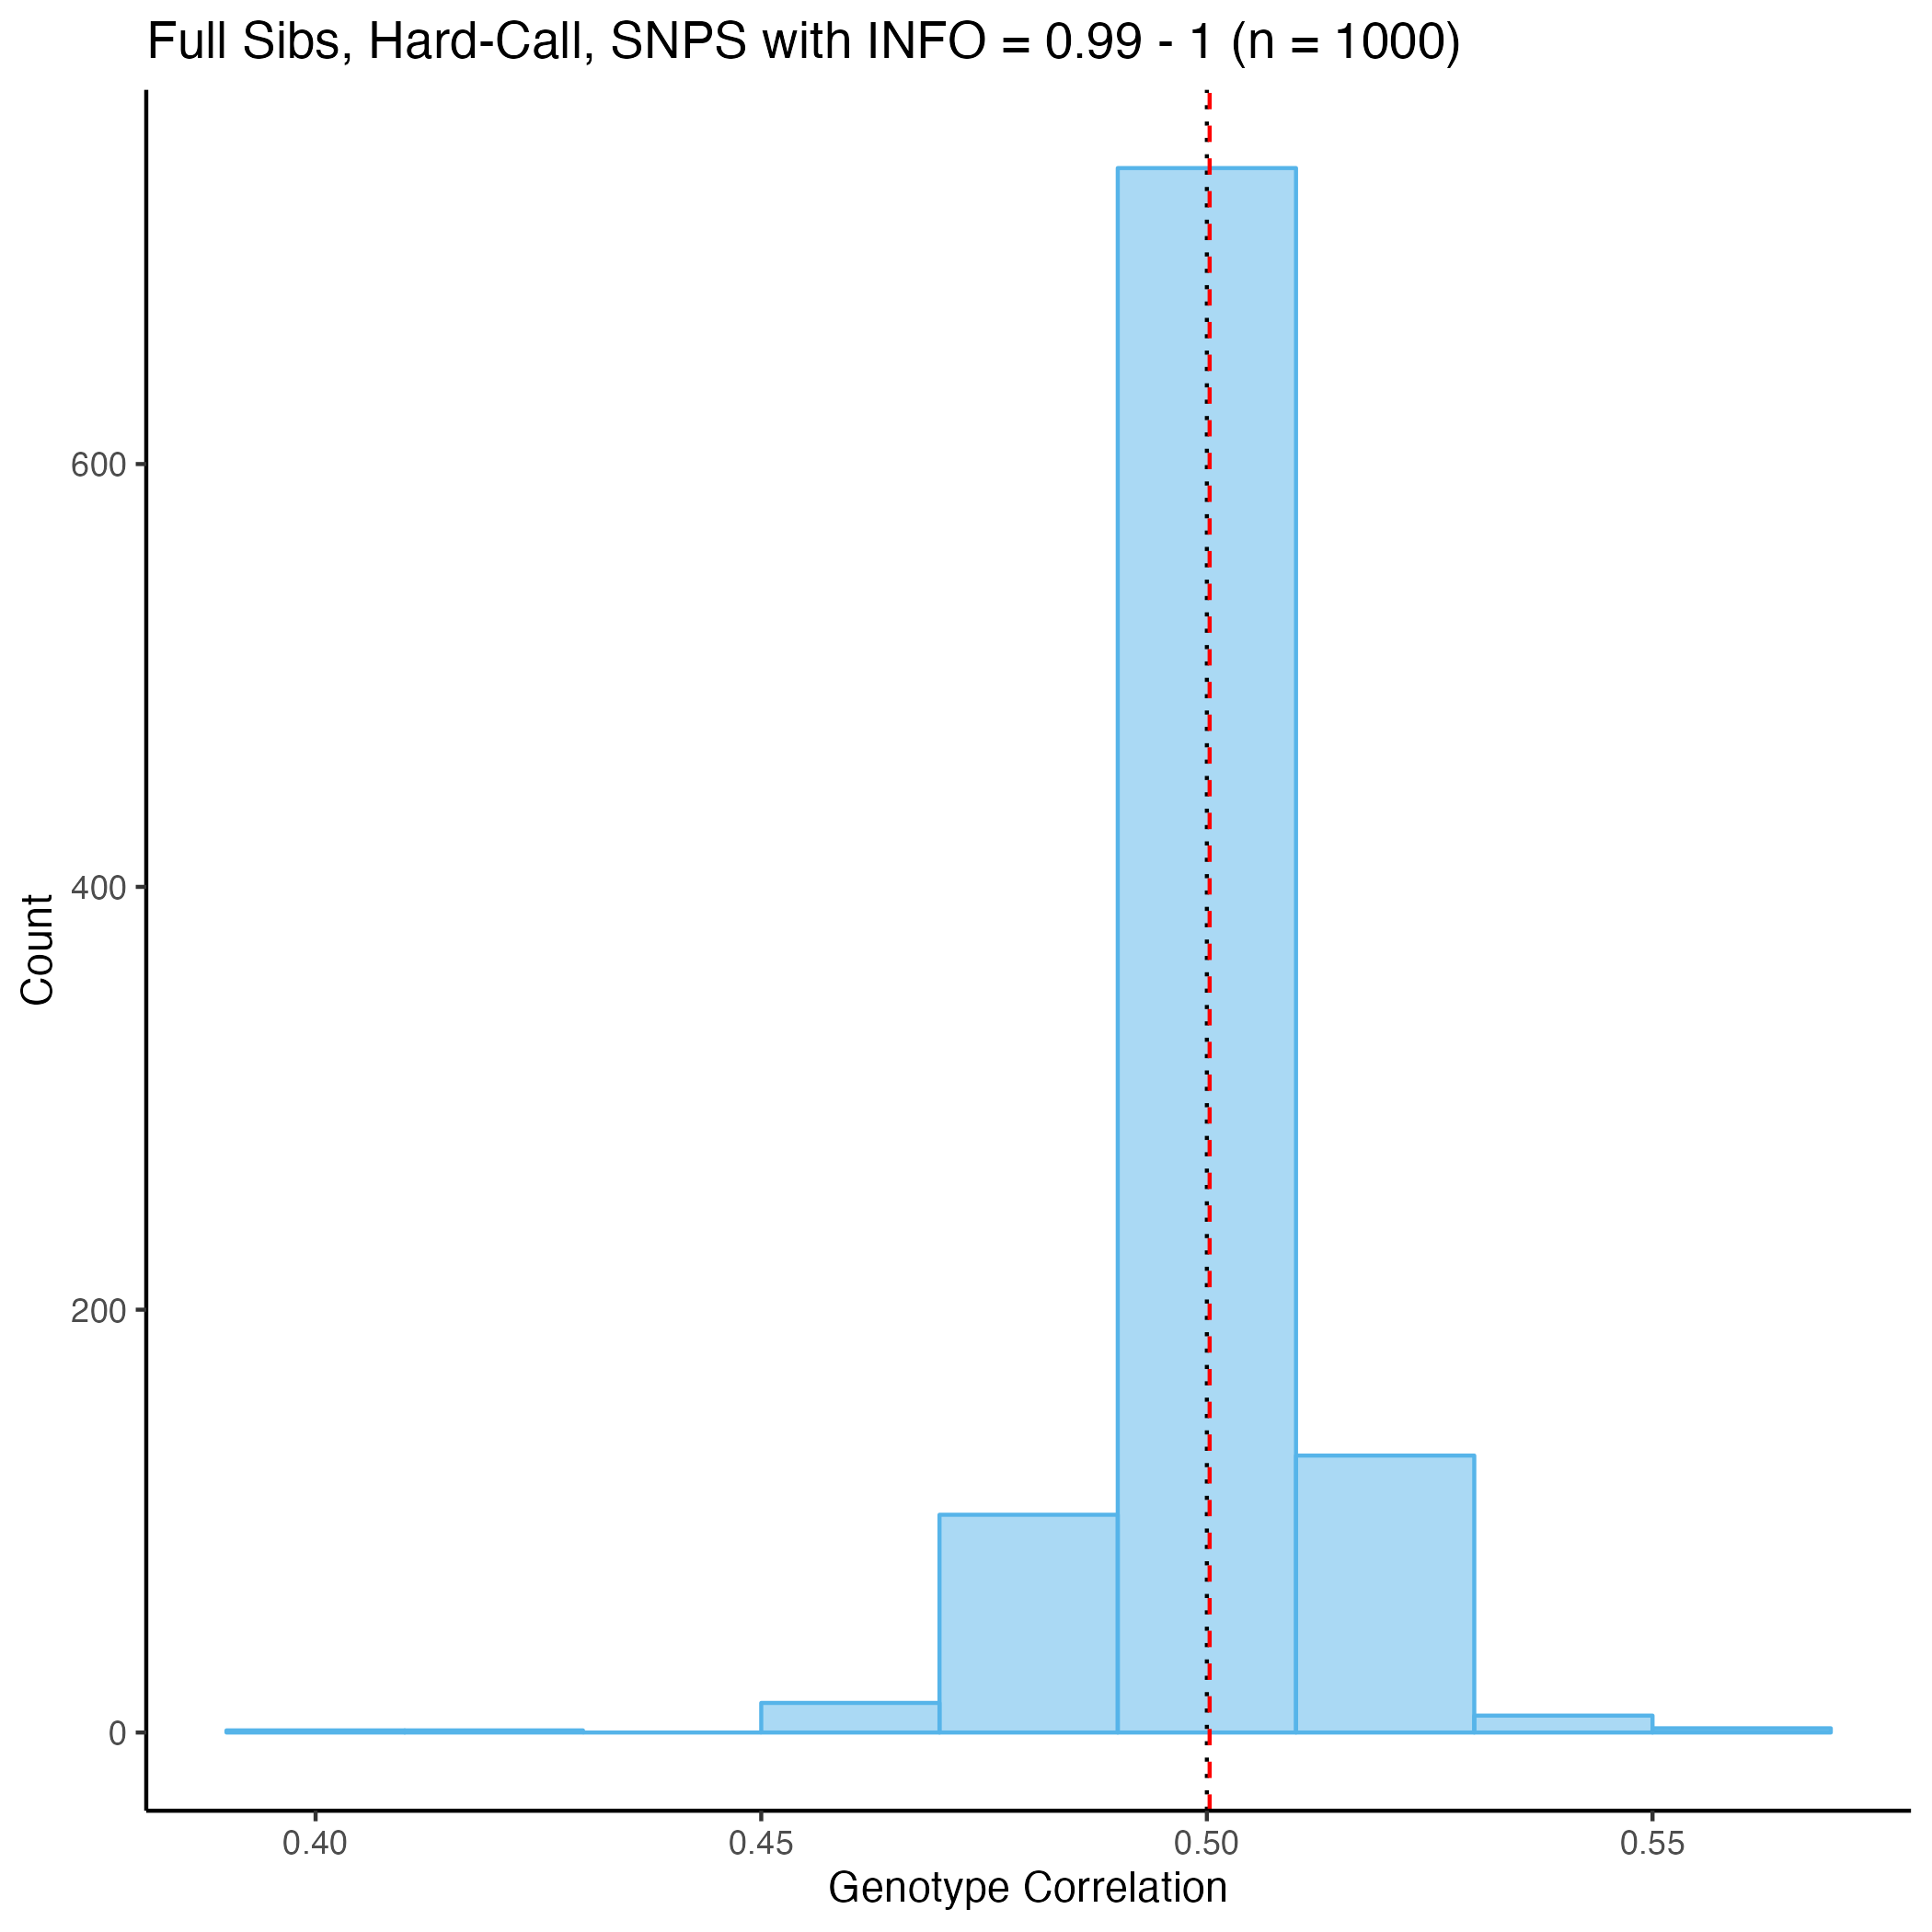
\includegraphics[width= .7\textwidth]{fig/FS-HC-i99.png}
            
\end{frame}



\begin{frame}{Correlations Distribution}{Low Quality SNPs - Full Siblings - Dosages}
      
      \centering         
      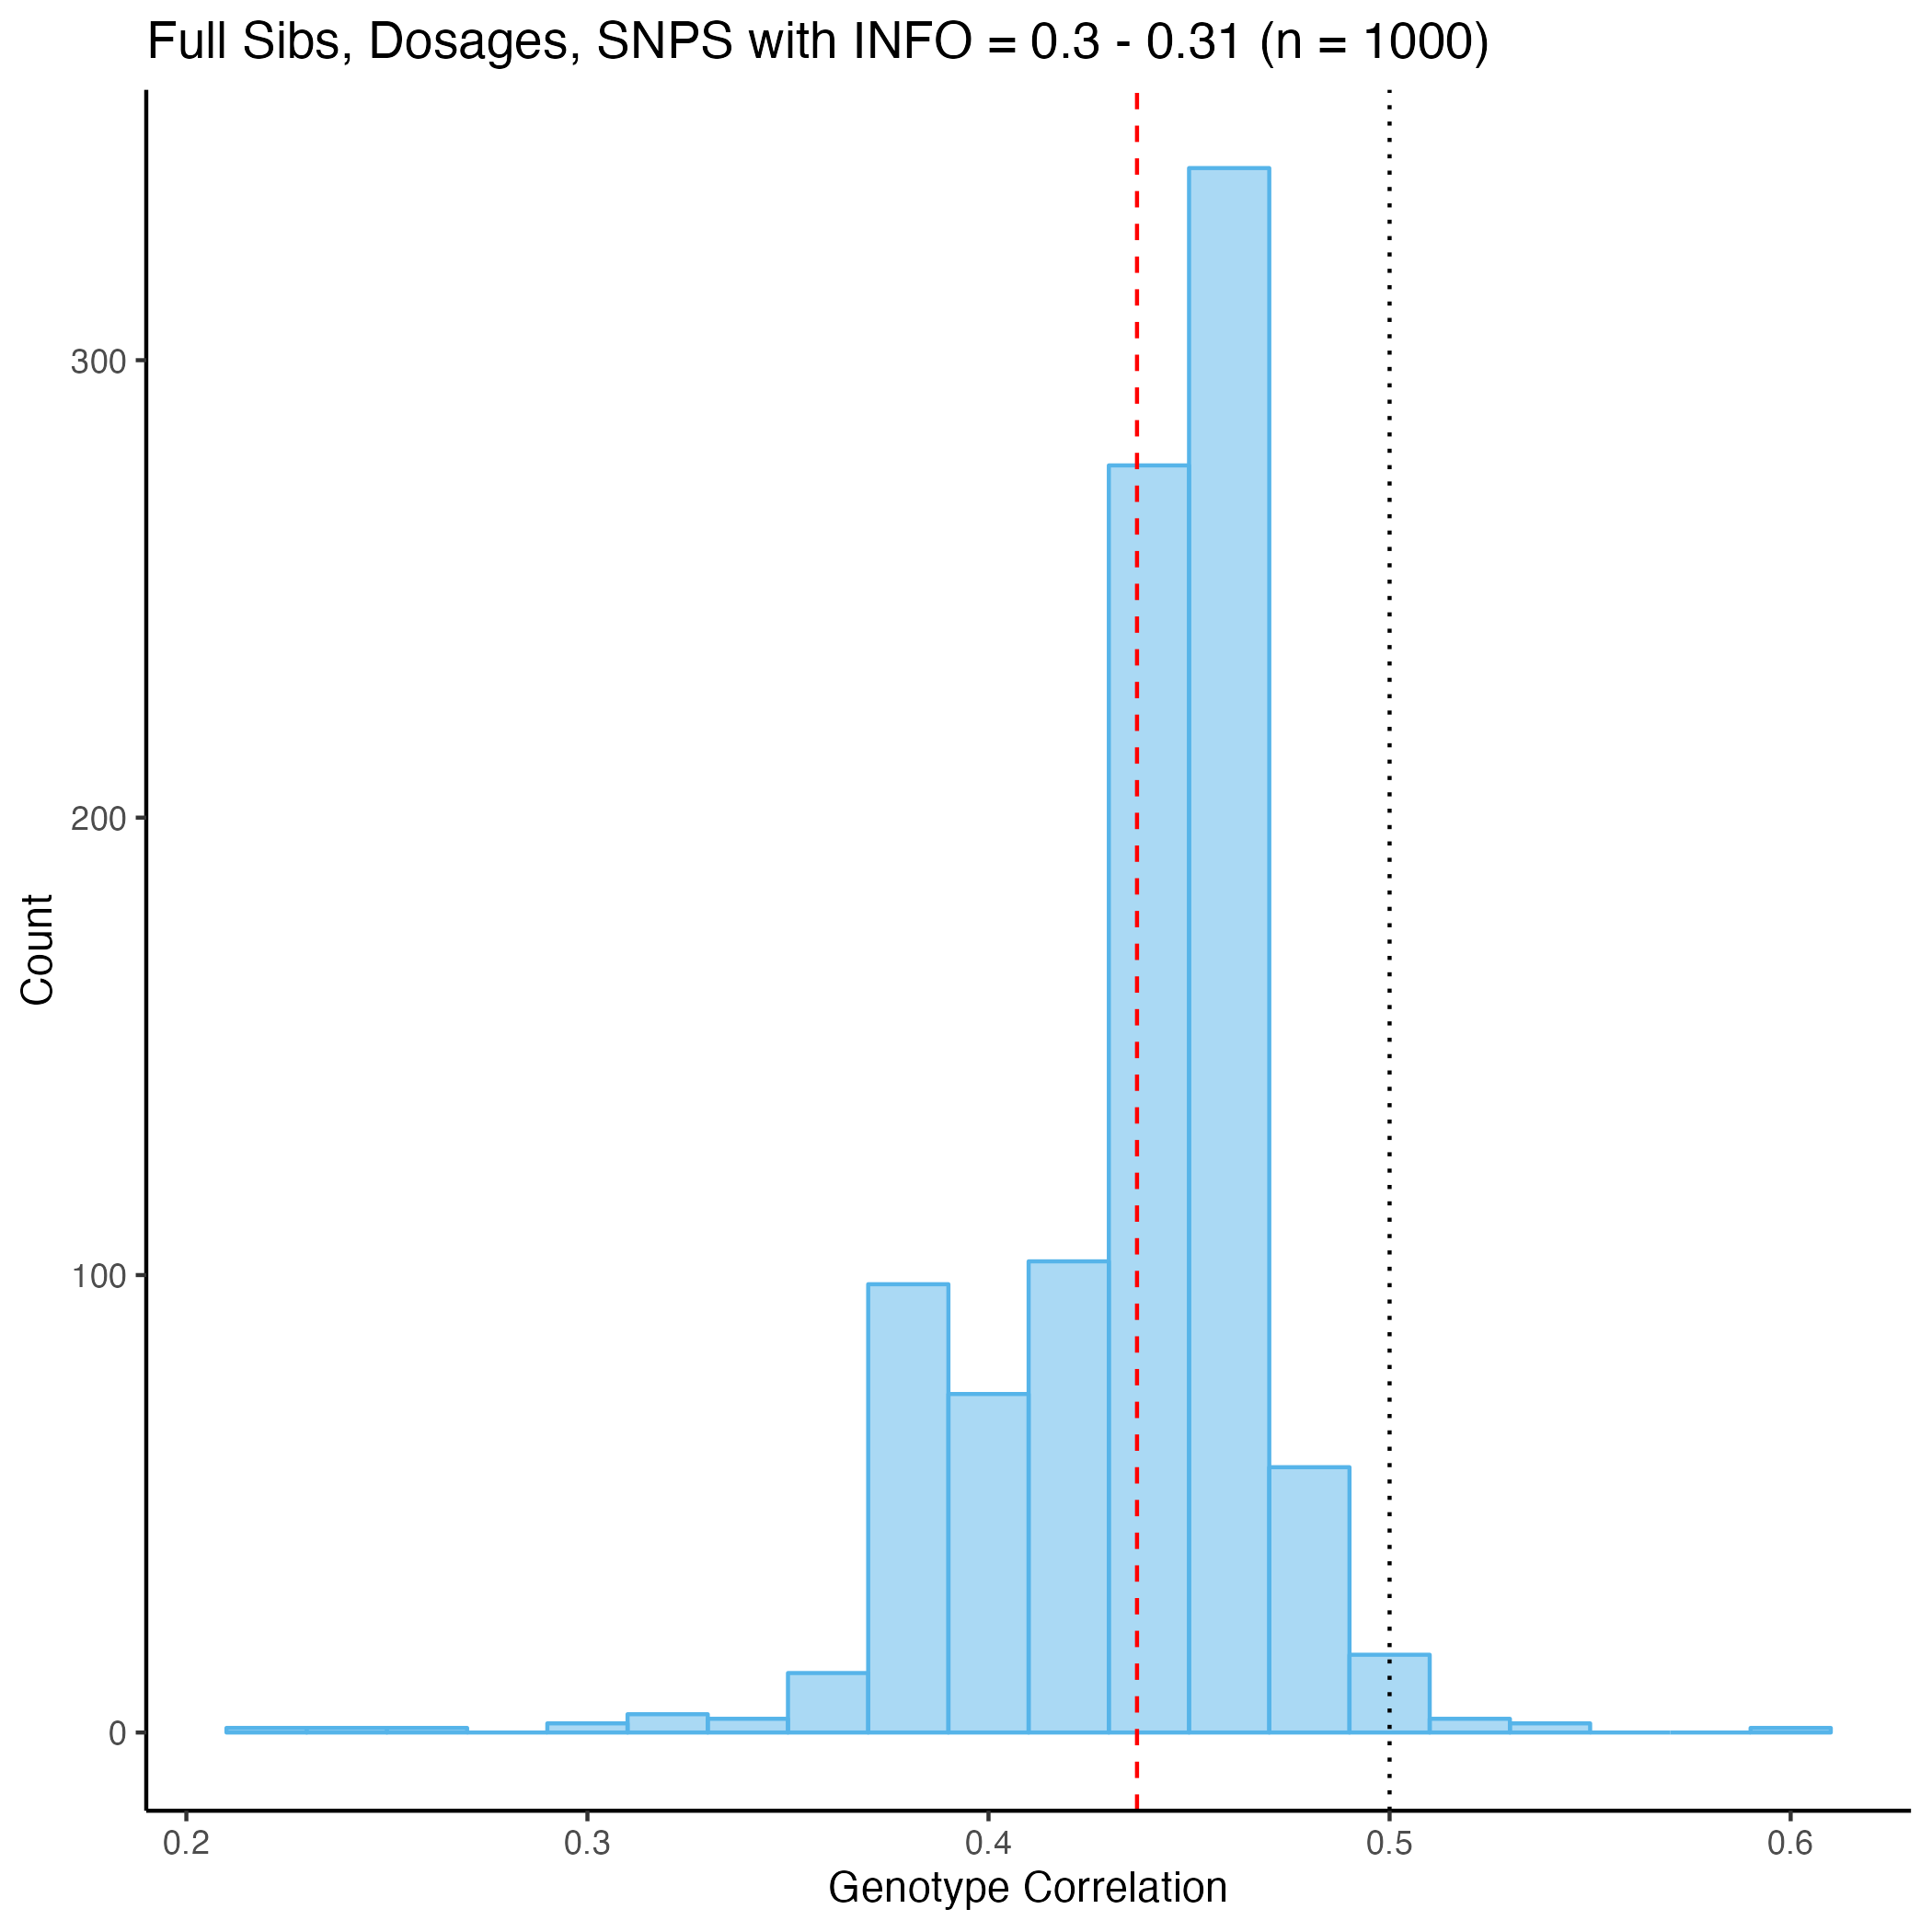
\includegraphics[width= .7\textwidth]{fig/FS-DSG-i30.png}
      
\end{frame}



\begin{frame}{Correlations Distribution}{Low Quality SNPs - Full Siblings - Hard Calls}
      
      \centering      
      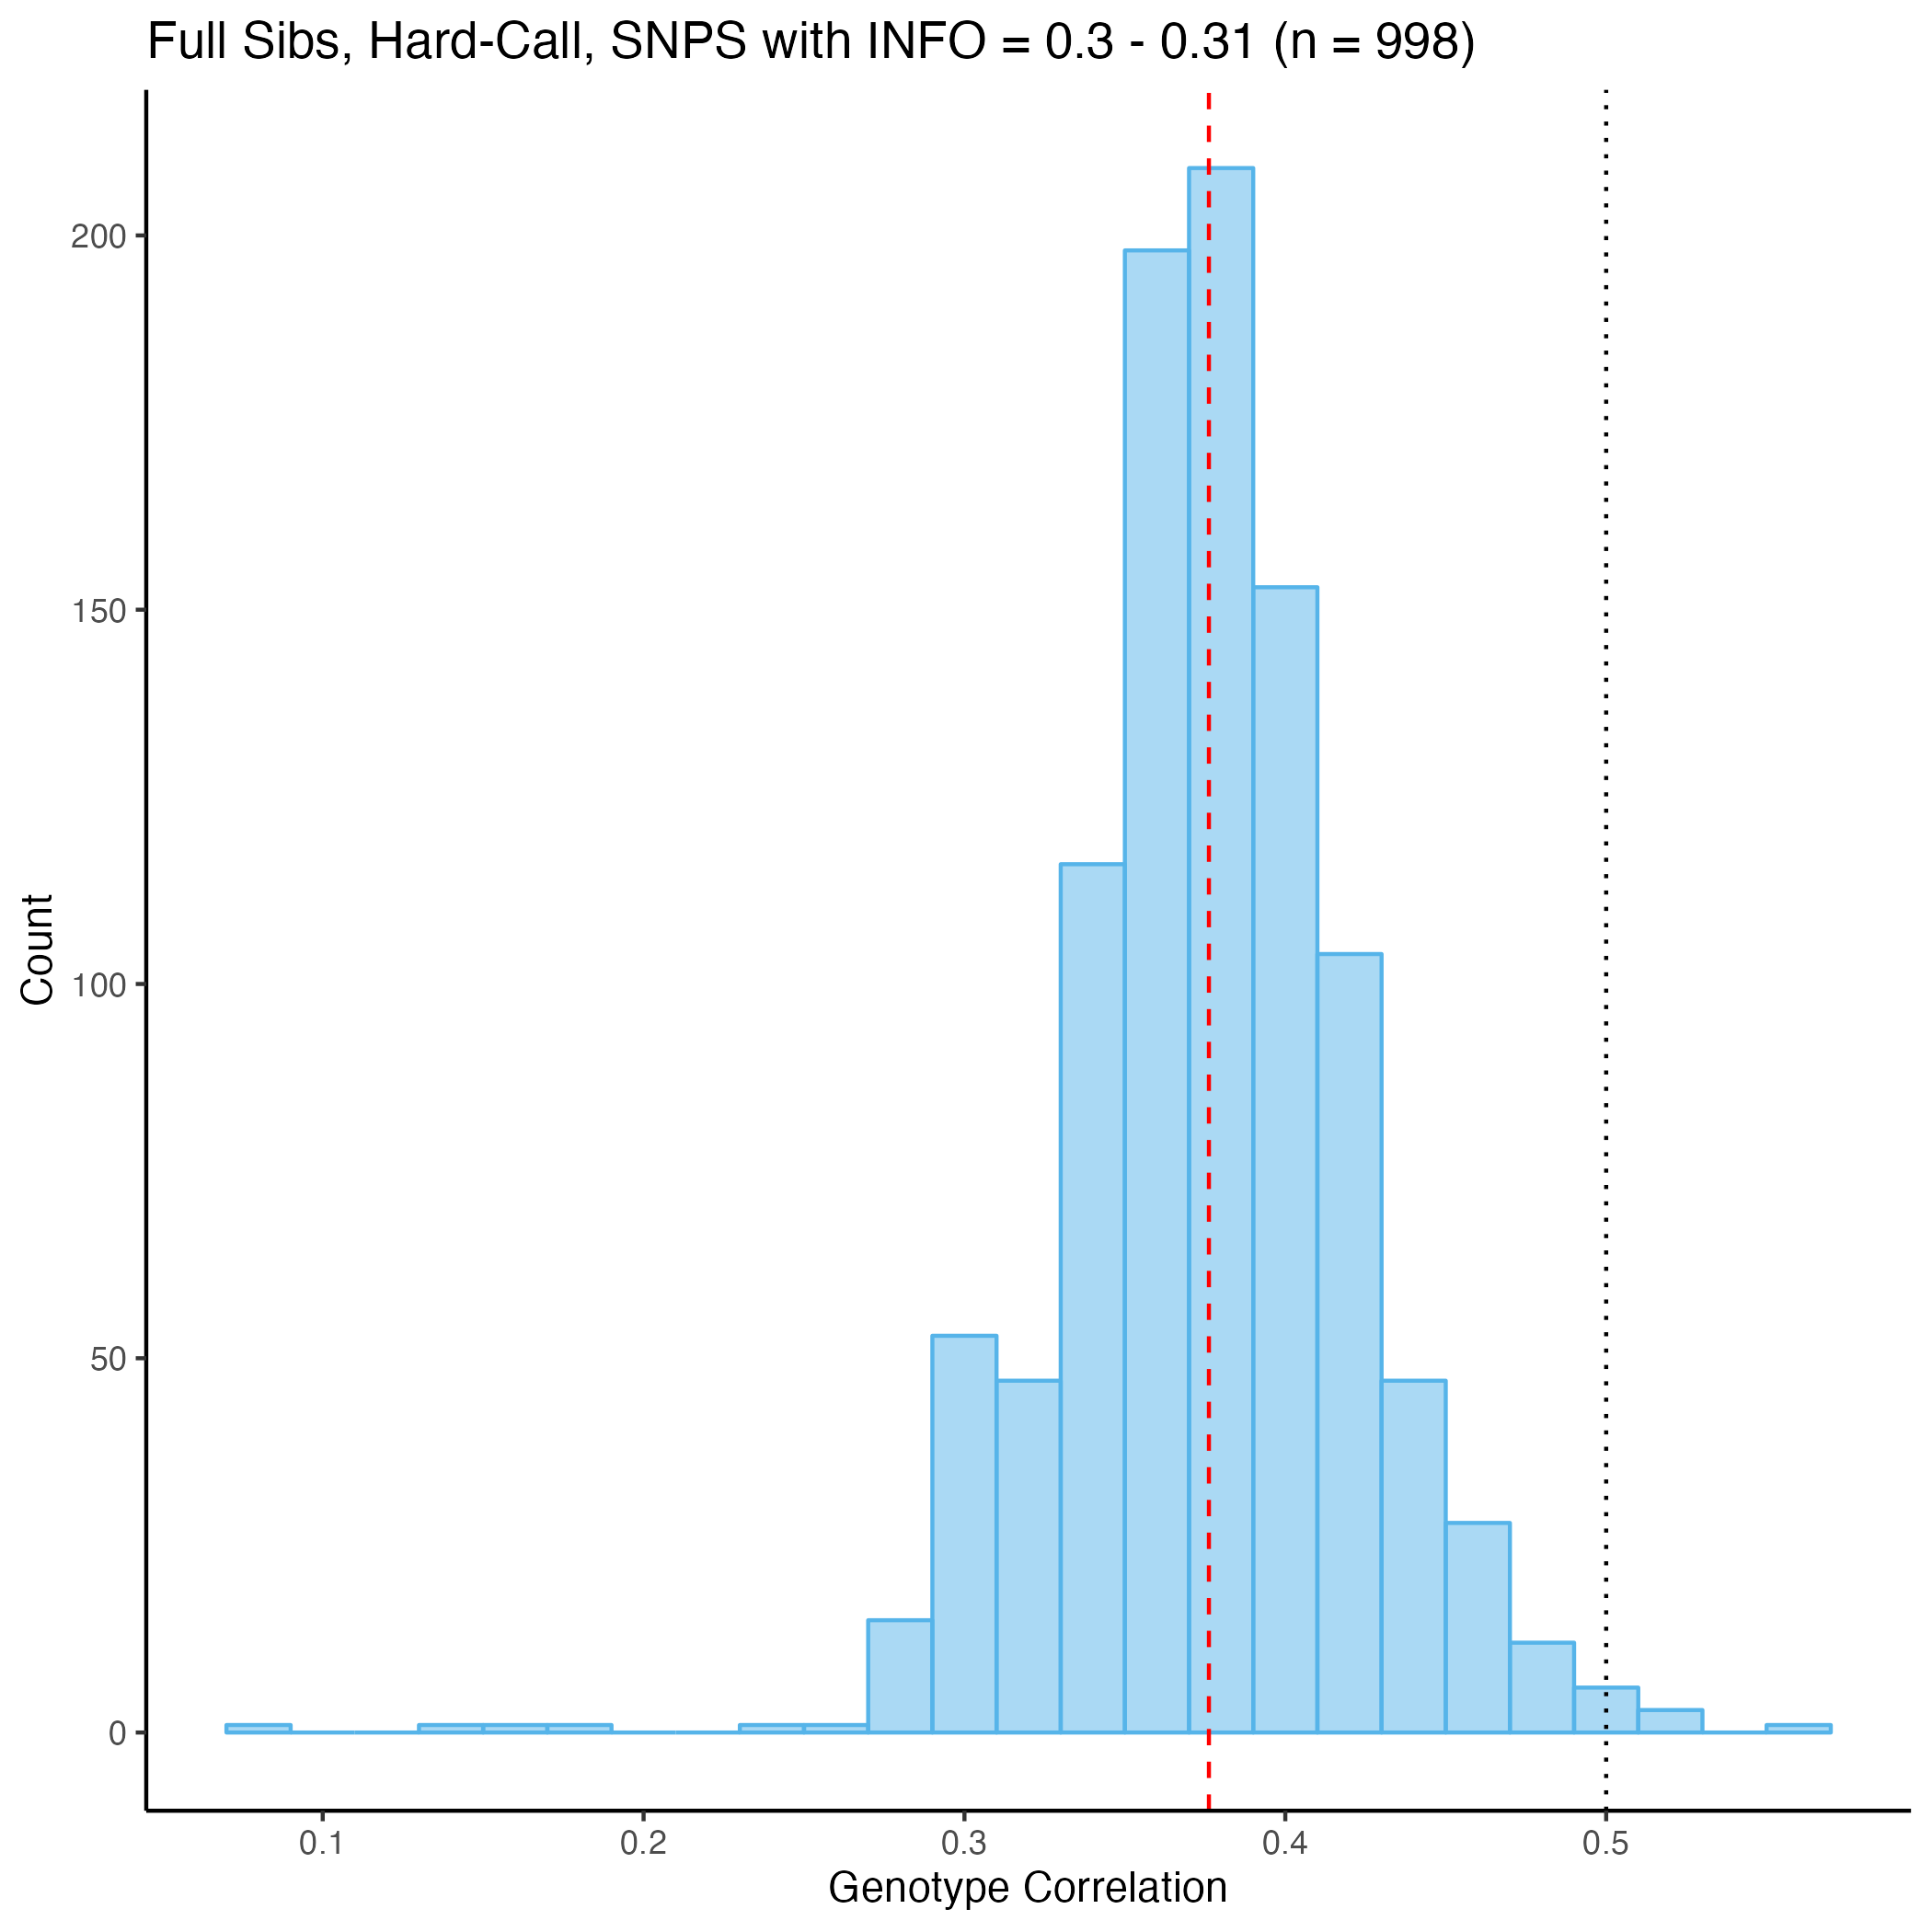
\includegraphics[width= .7\textwidth]{fig/FS-HC-i30.png}
            
\end{frame}

% We also have the sampe pattern for the parent-offspring pairs, I didn't make slide with those because they have similiar patterns
% out of 280 plots I chose these ones only to show the overall trend and issue.

% if we gather all those results and draw it as a function of info score we can see the trend more clearly 
% we have the mean of all those 280 plots on this plot all together.


% if we put all these 
% The correlation decreases as the info score decreases below one
% This is ture for both dosages and hard calls for both siblings and parent-offspring pairs.
% the drop in correlation is much steeper for hard calls. 
% remember Howe etal used Hard call and the situation is worse for hard calls

% both dosages and hard calls exihibit this behavior and this is not what we expect them and it is worse
% for hard calls than dosages

% and parent-offspring pairs & siblings pairs are basically the same for dosages
% but it is worse for parent-offspring pairs when using hard-calls

\begin{frame}{Mean Genotype Correlation}{As a function of Info Score}

      \centering
      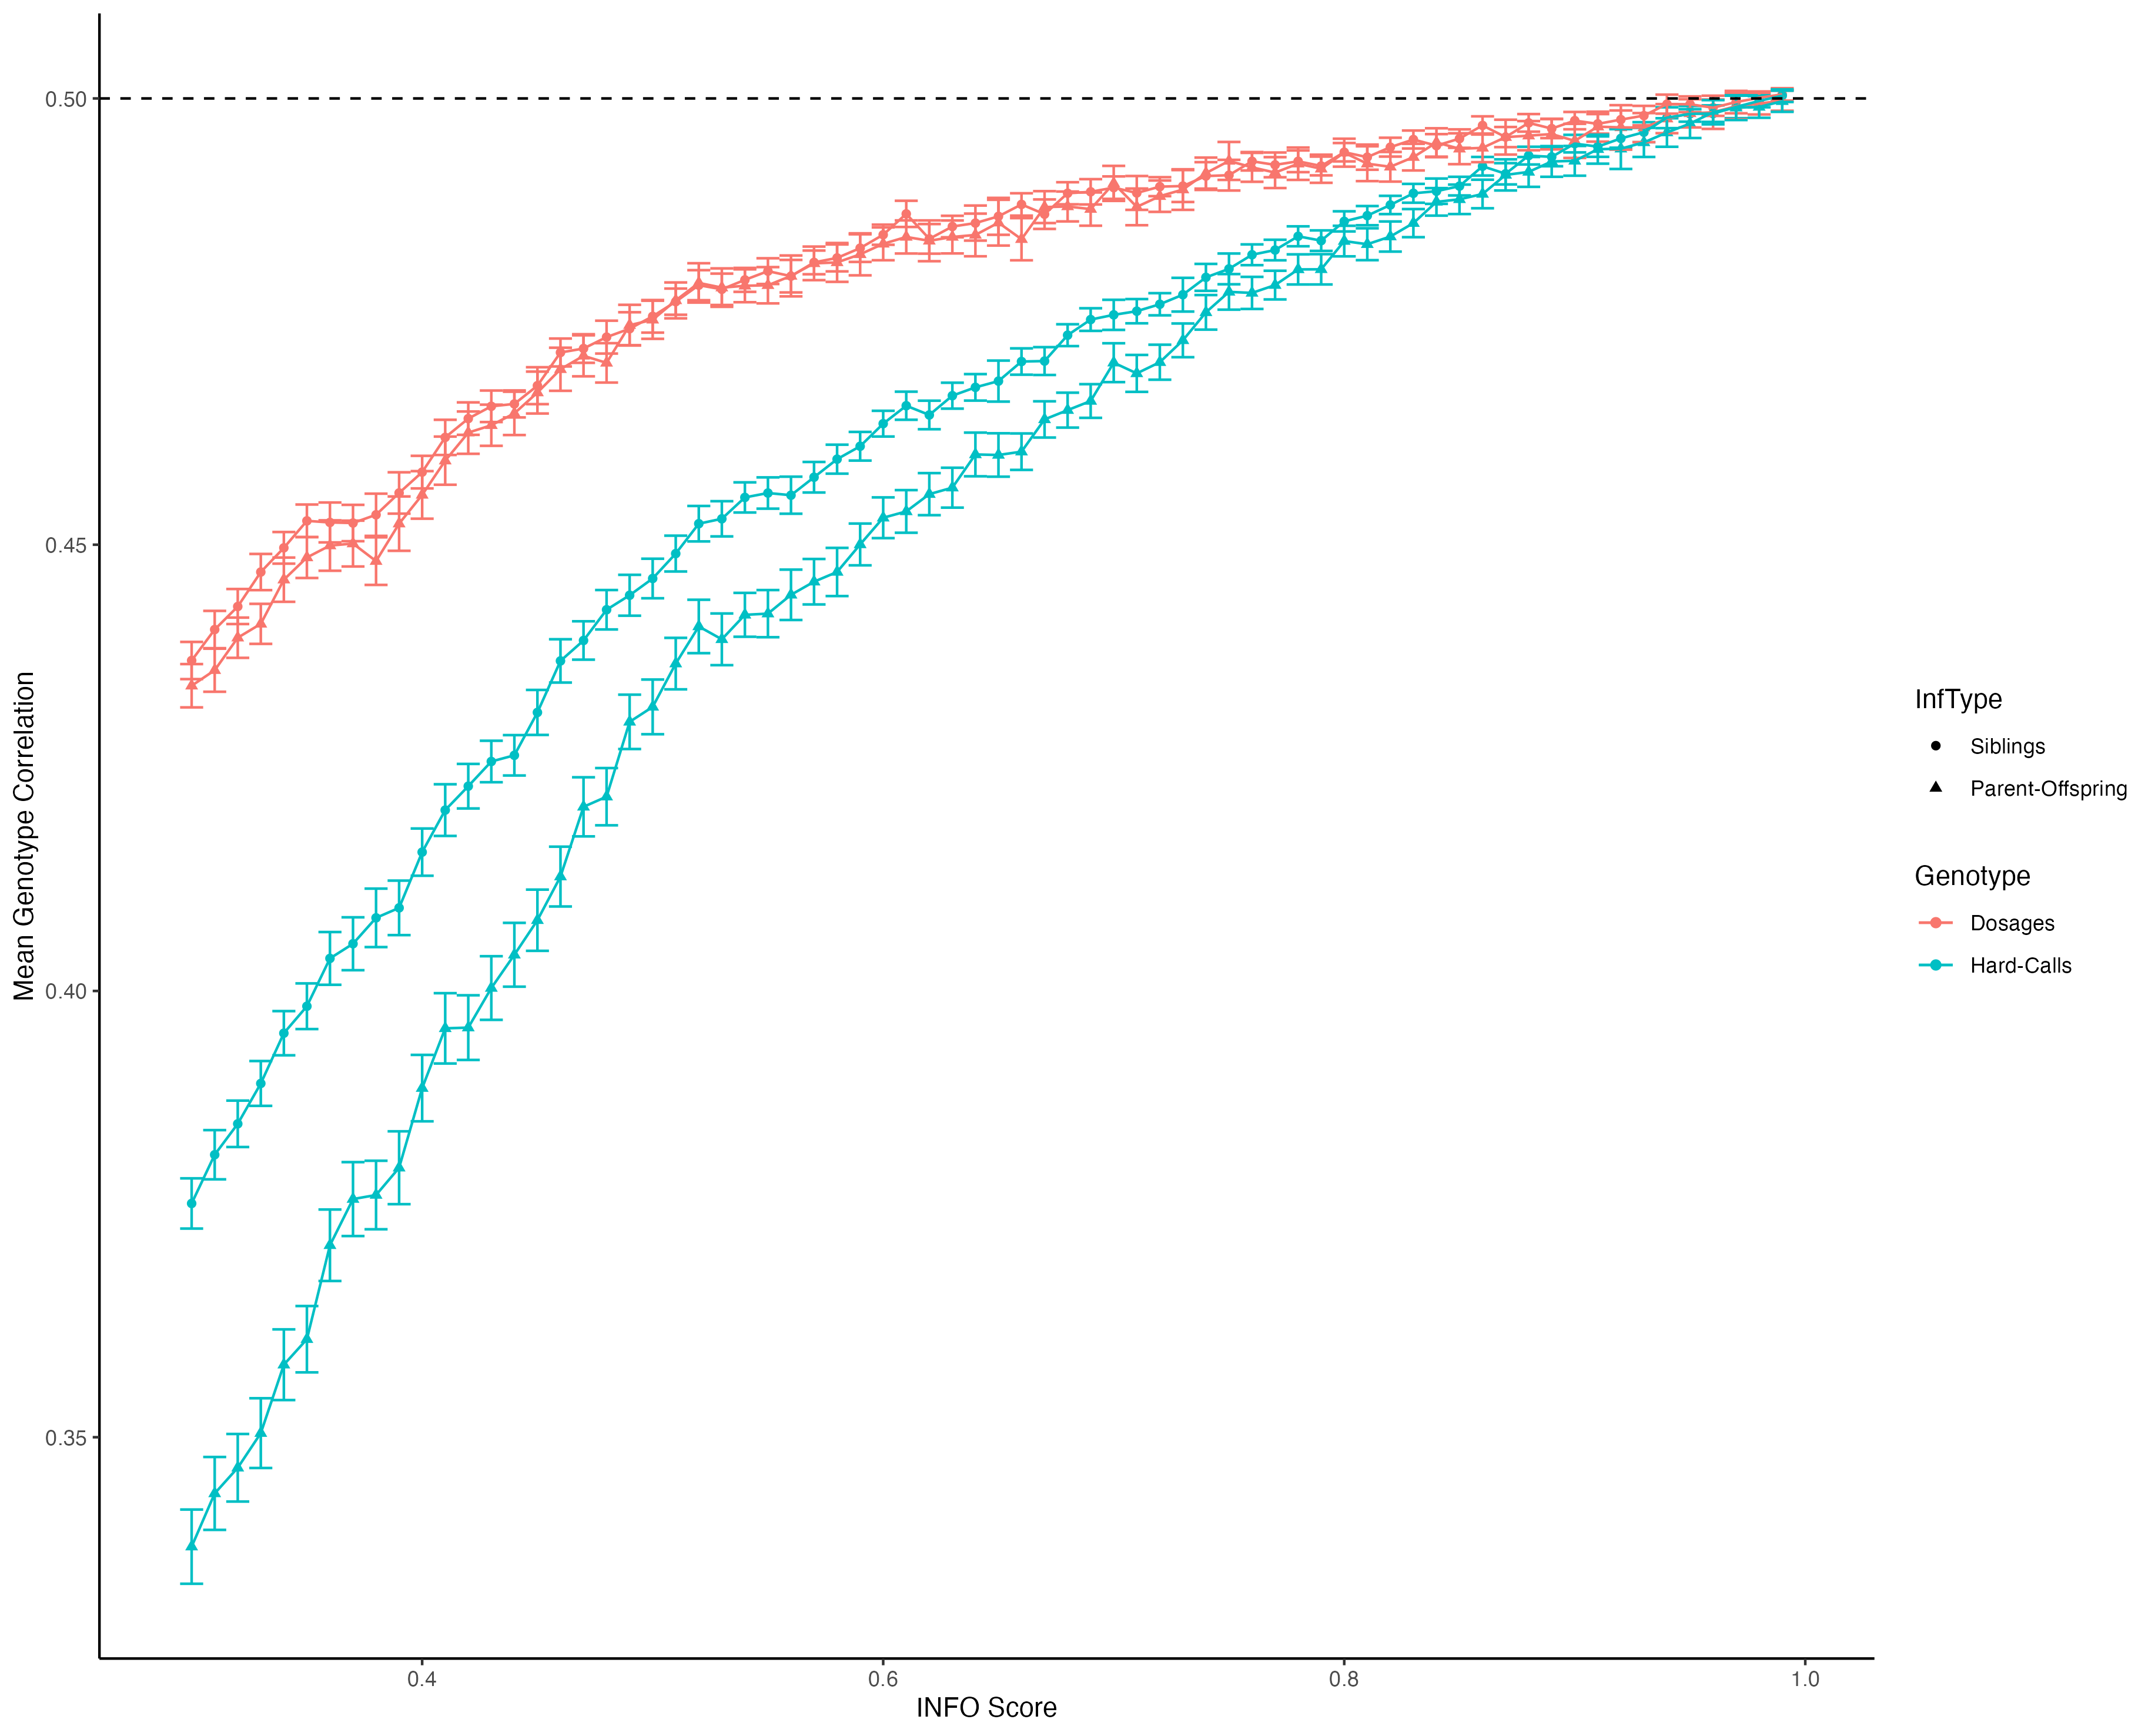
\includegraphics[width=.9\textwidth]{fig/mean_gt_corr_v2.png}
      
\end{frame}



\section{Correlation Analysis Conditional on IBD states}

% add formulas here

\begin{frame}{Correlation Analysis Conditional on IBD states}
    

\begin{itemize}
    \item What if we calculate all these correlations conditional on IBD states?
    \item Conditioning on IBD states for parent-offspring pairs doesn't mean anything because they are always IBD = 1 so we would get the same results as before when we didn't condition on IBD states.
    \item Suppose \(i\) and \(j\) are siblings. Then in theory we have

\end{itemize}


\[
      Corr(G_i, G_j | IBD = 0) = 0
\]

% the same for one parent but different from the other parent

\[
      Corr(G_i, G_j | IBD = 1) = 0.5
\]

% when IBD is 2 it means that in that part of the genome both paternal & maternal side of
% the genome is the same for that siblings pairs. So they are inheriting the same from both parents.


\[
      Corr(G_i, G_j | IBD = 2) = 1
\]


\end{frame}




% \begin{frame}{Correlations Dist. Conditional on IBD states}{Low Quality SNP - Full Siblings - Dosages - IBD = 0}

% \begin{figure}

%       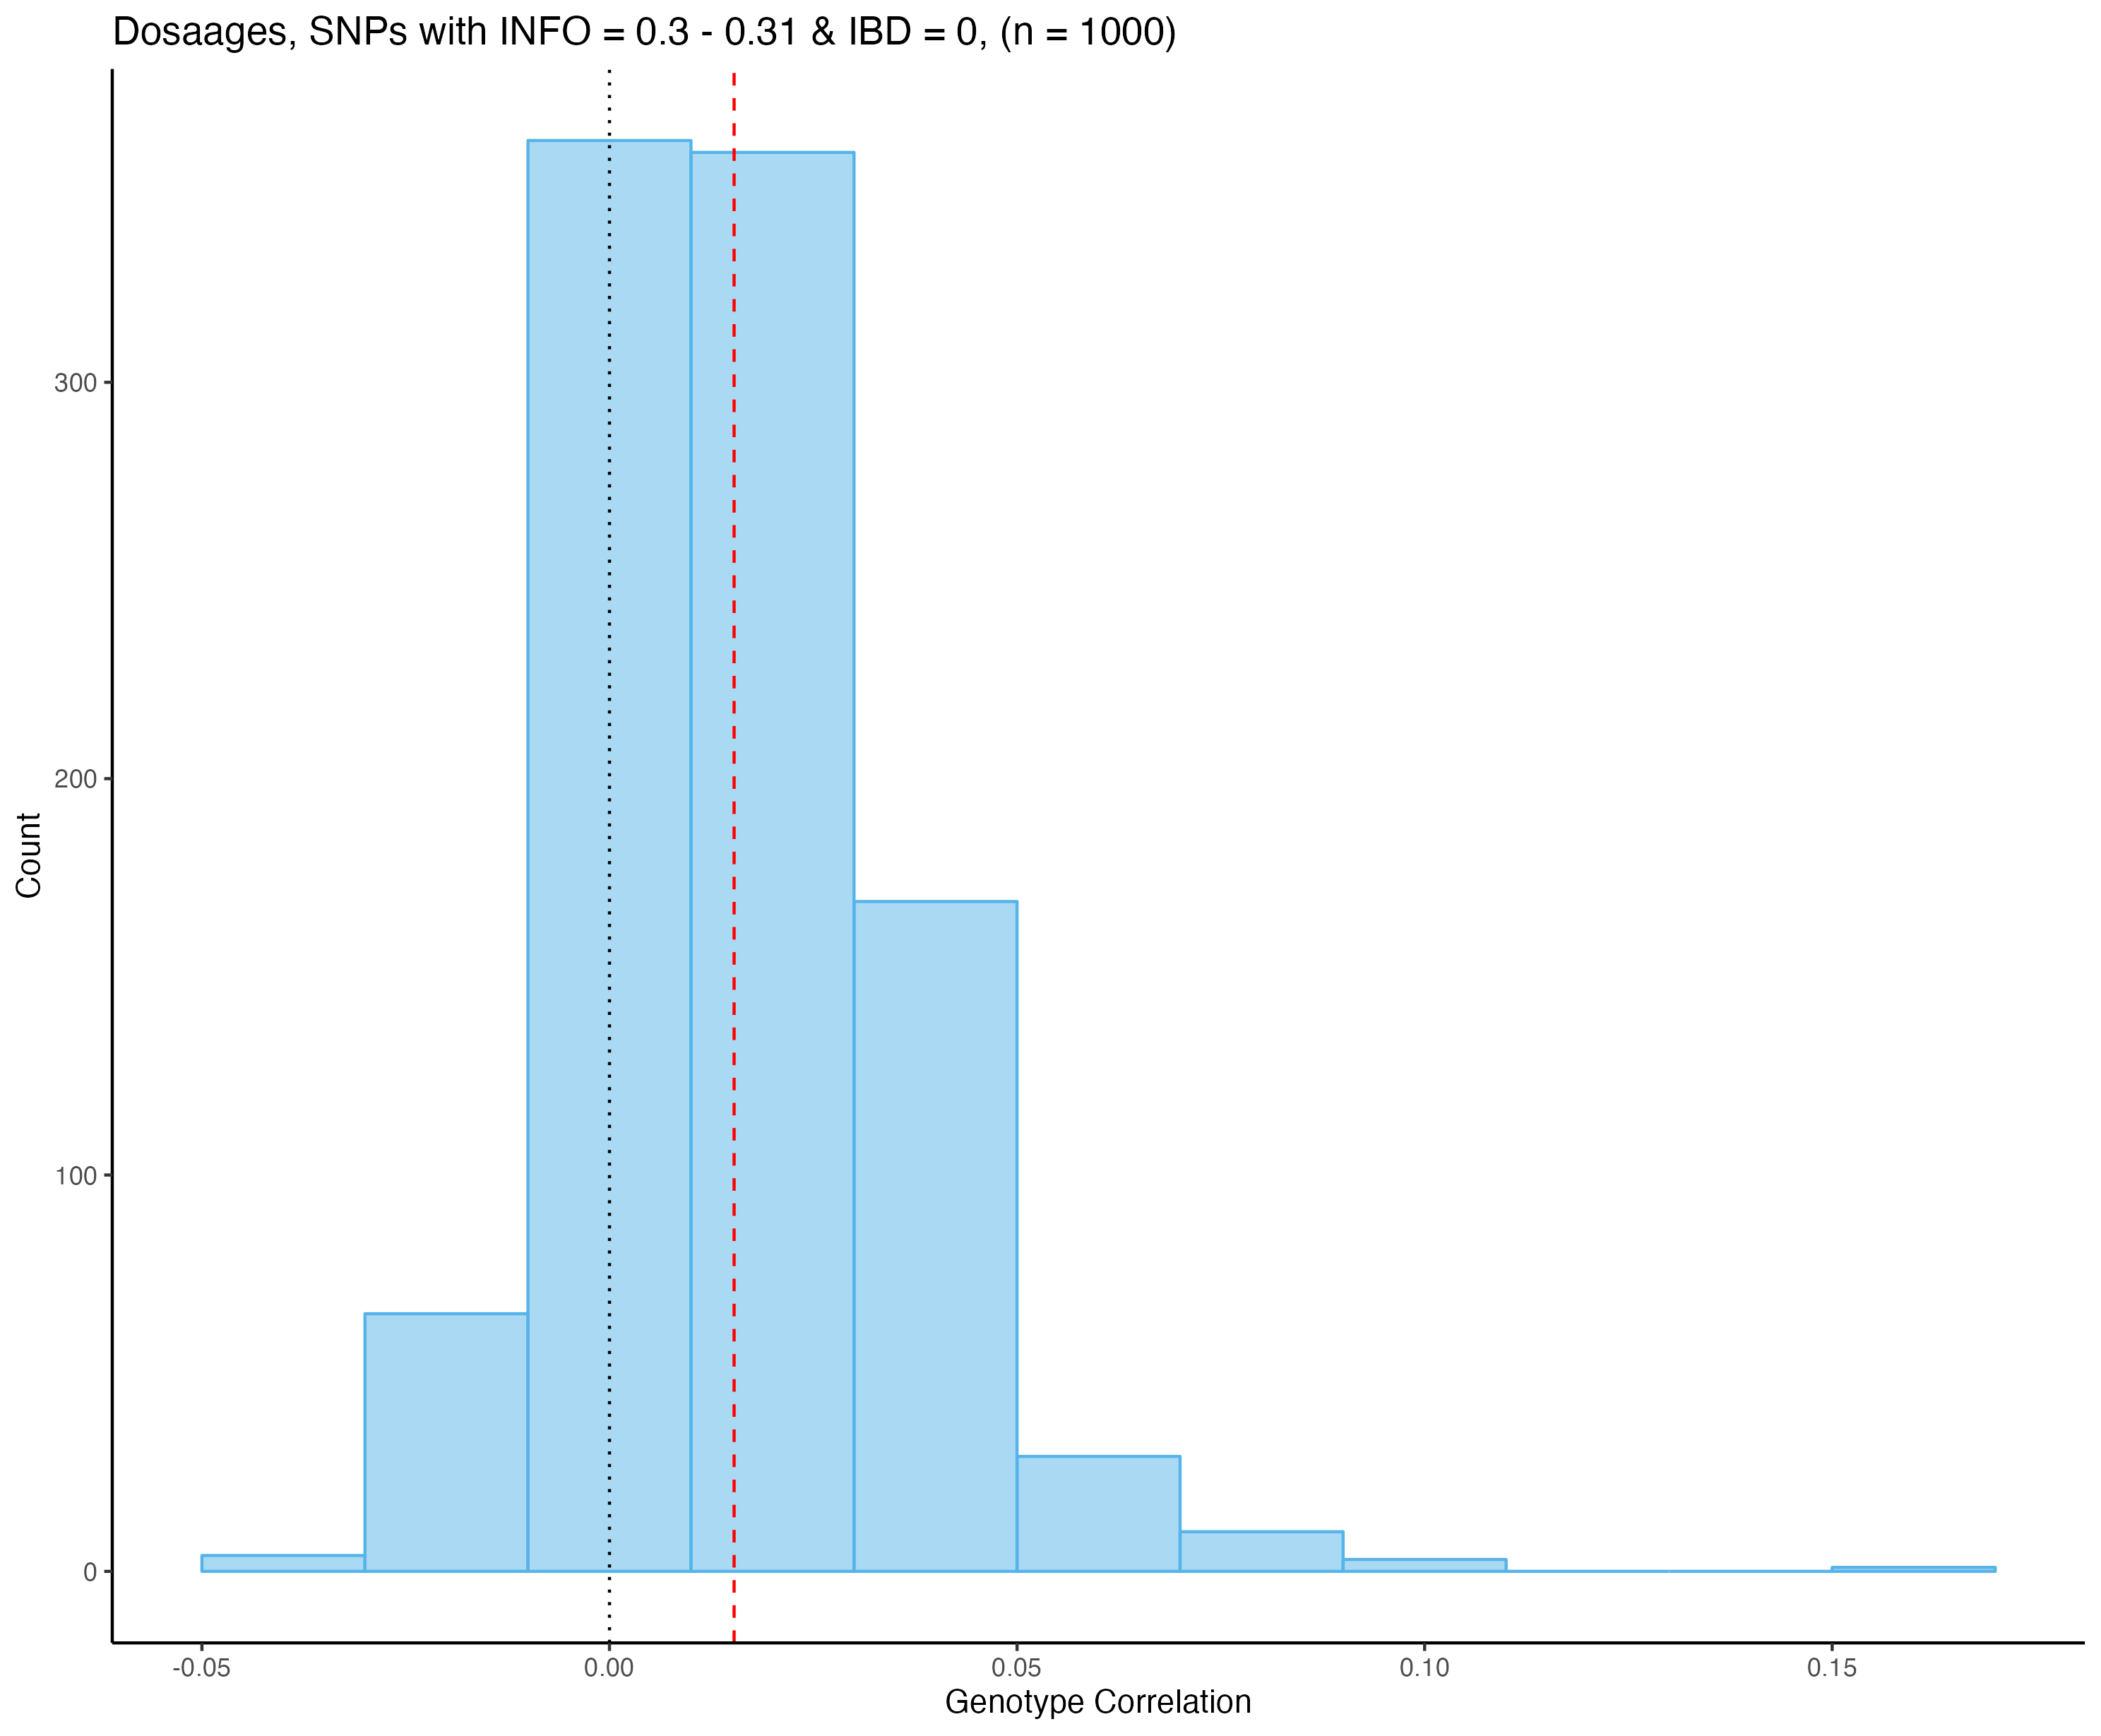
\includegraphics[width= .85\textwidth]{fig/DS-0-i30.png}
      
% \end{figure}

% \end{frame}




% \begin{frame}{Correlations Dist. Conditional on IBD states}{Low Quality SNP - Full Siblings - Dosages - IBD = 1}

% \begin{figure}

%       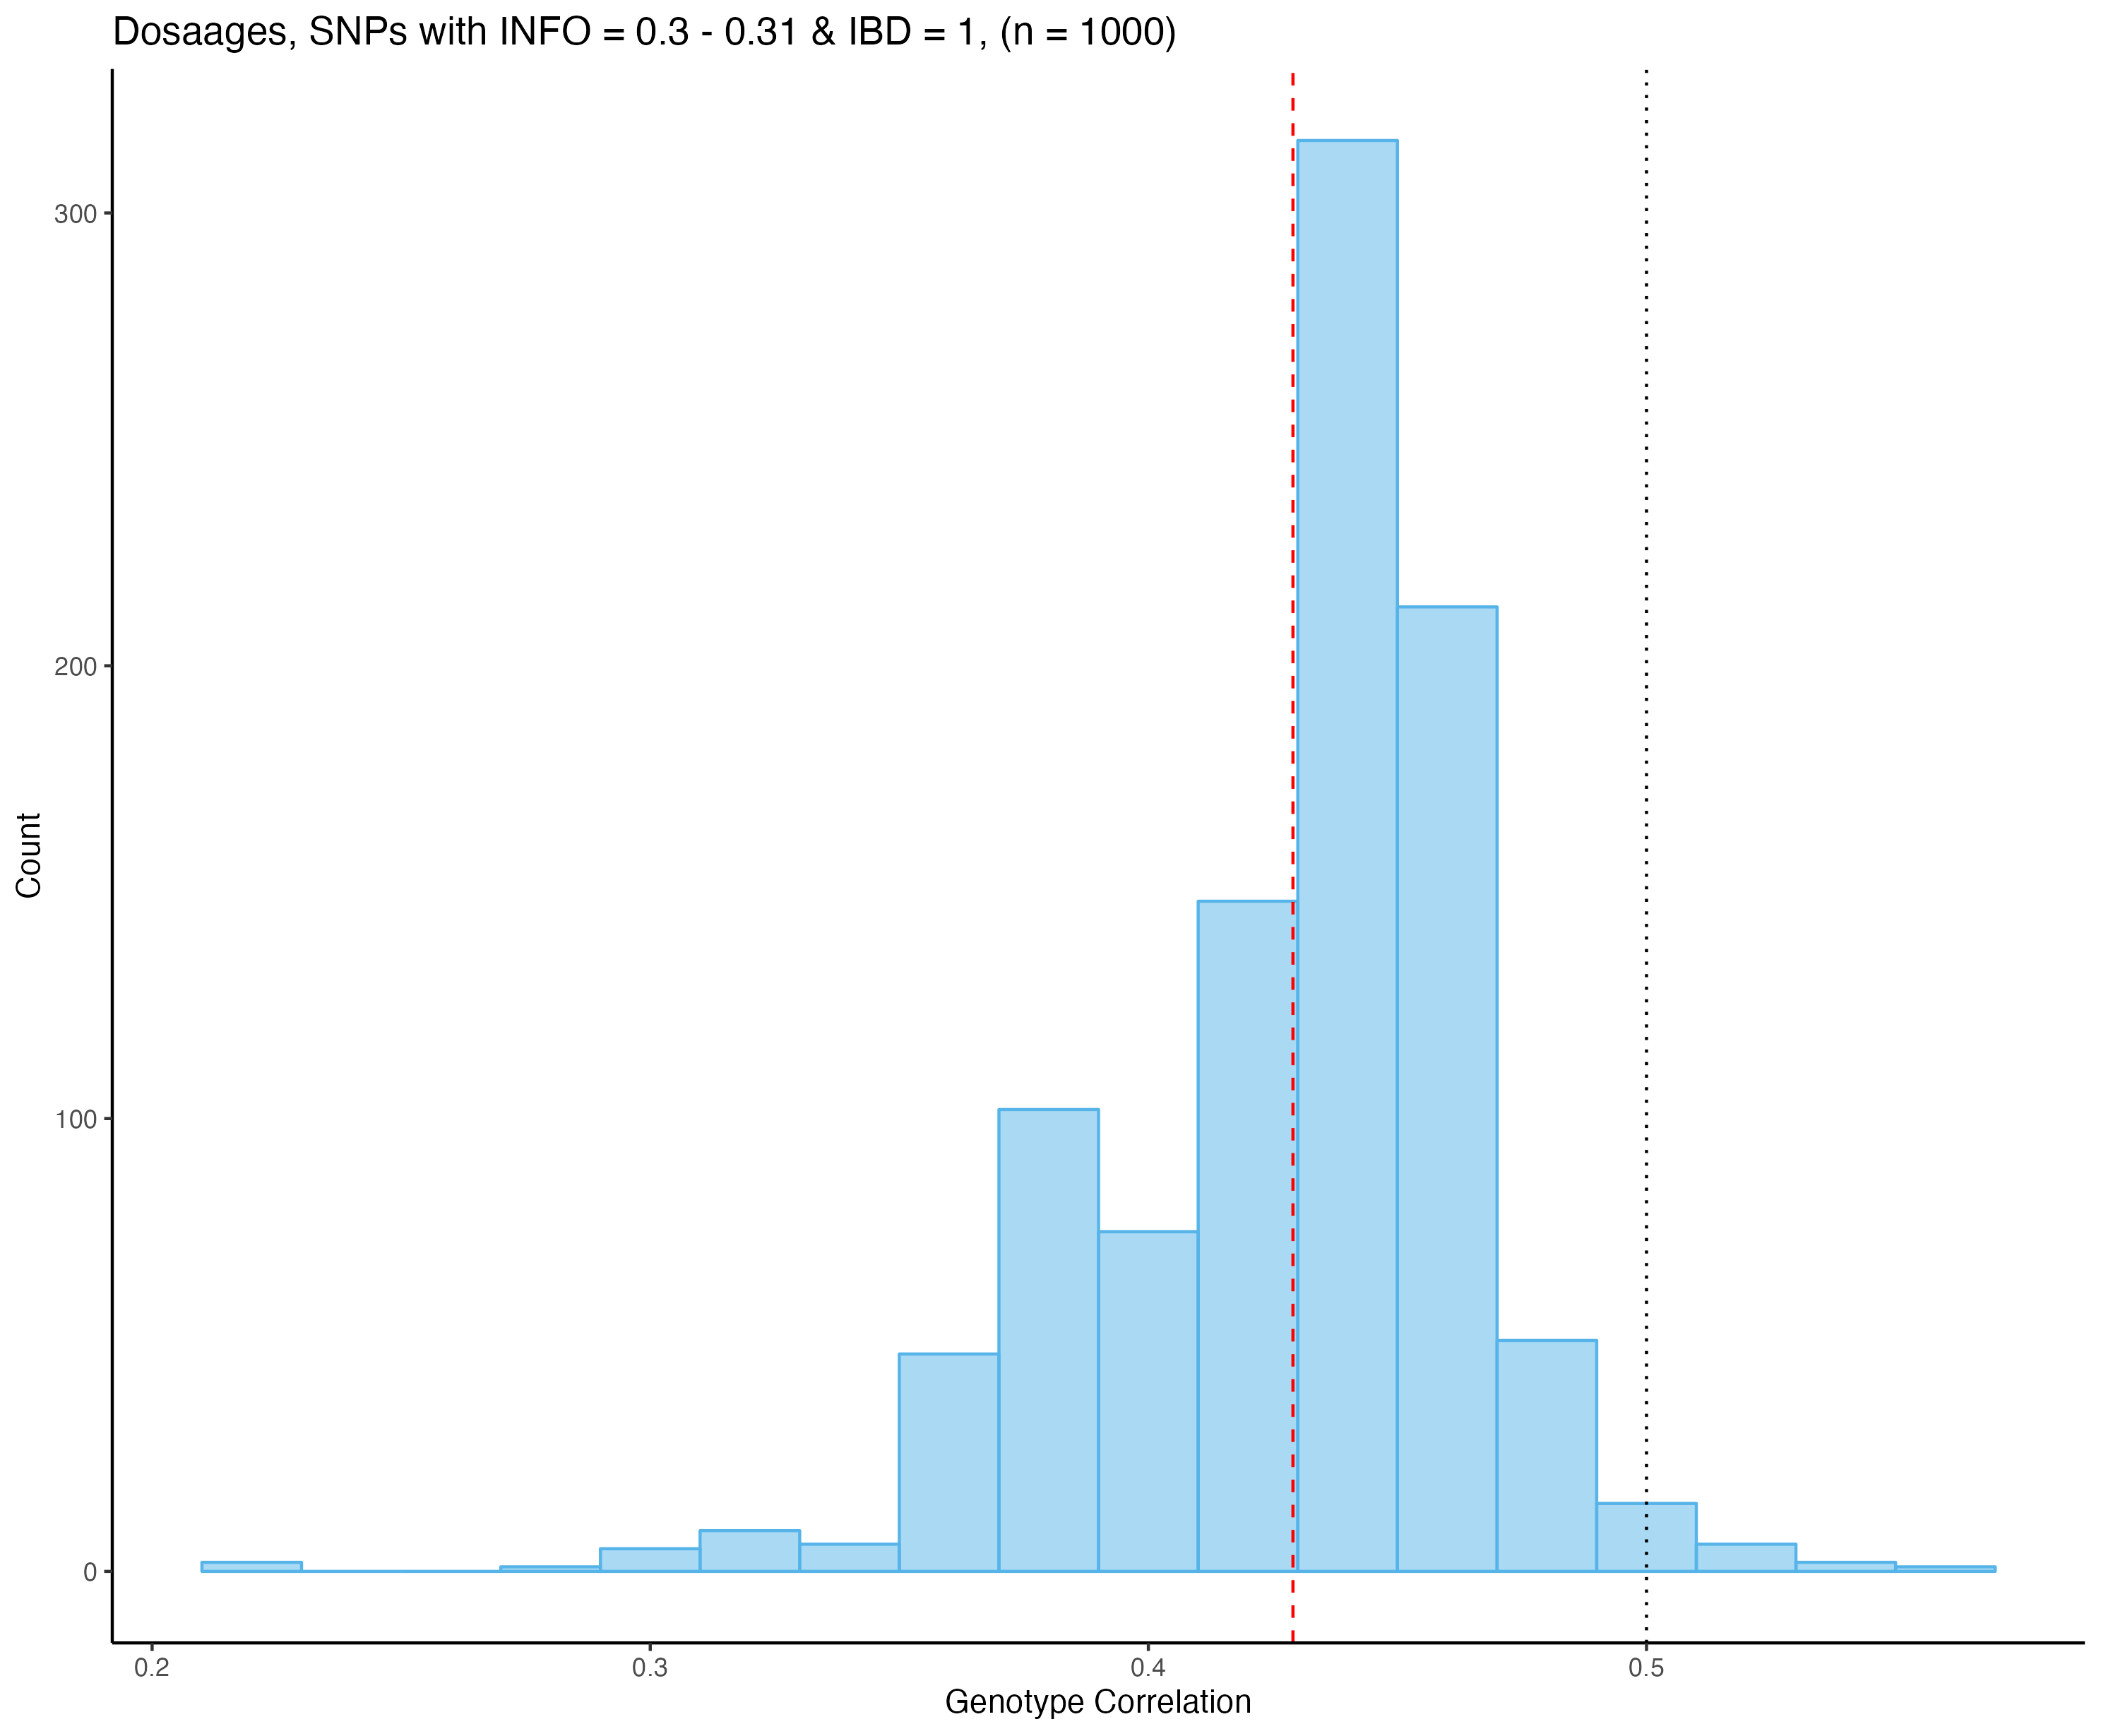
\includegraphics[width= .85\textwidth]{fig/DS-1-i30.png}
      
% \end{figure}

% \end{frame}




\begin{frame}{Correlations Dist. Conditional on IBD states}{Low Quality SNP - Full Siblings - Dosages - IBD = 2}

\begin{figure}

      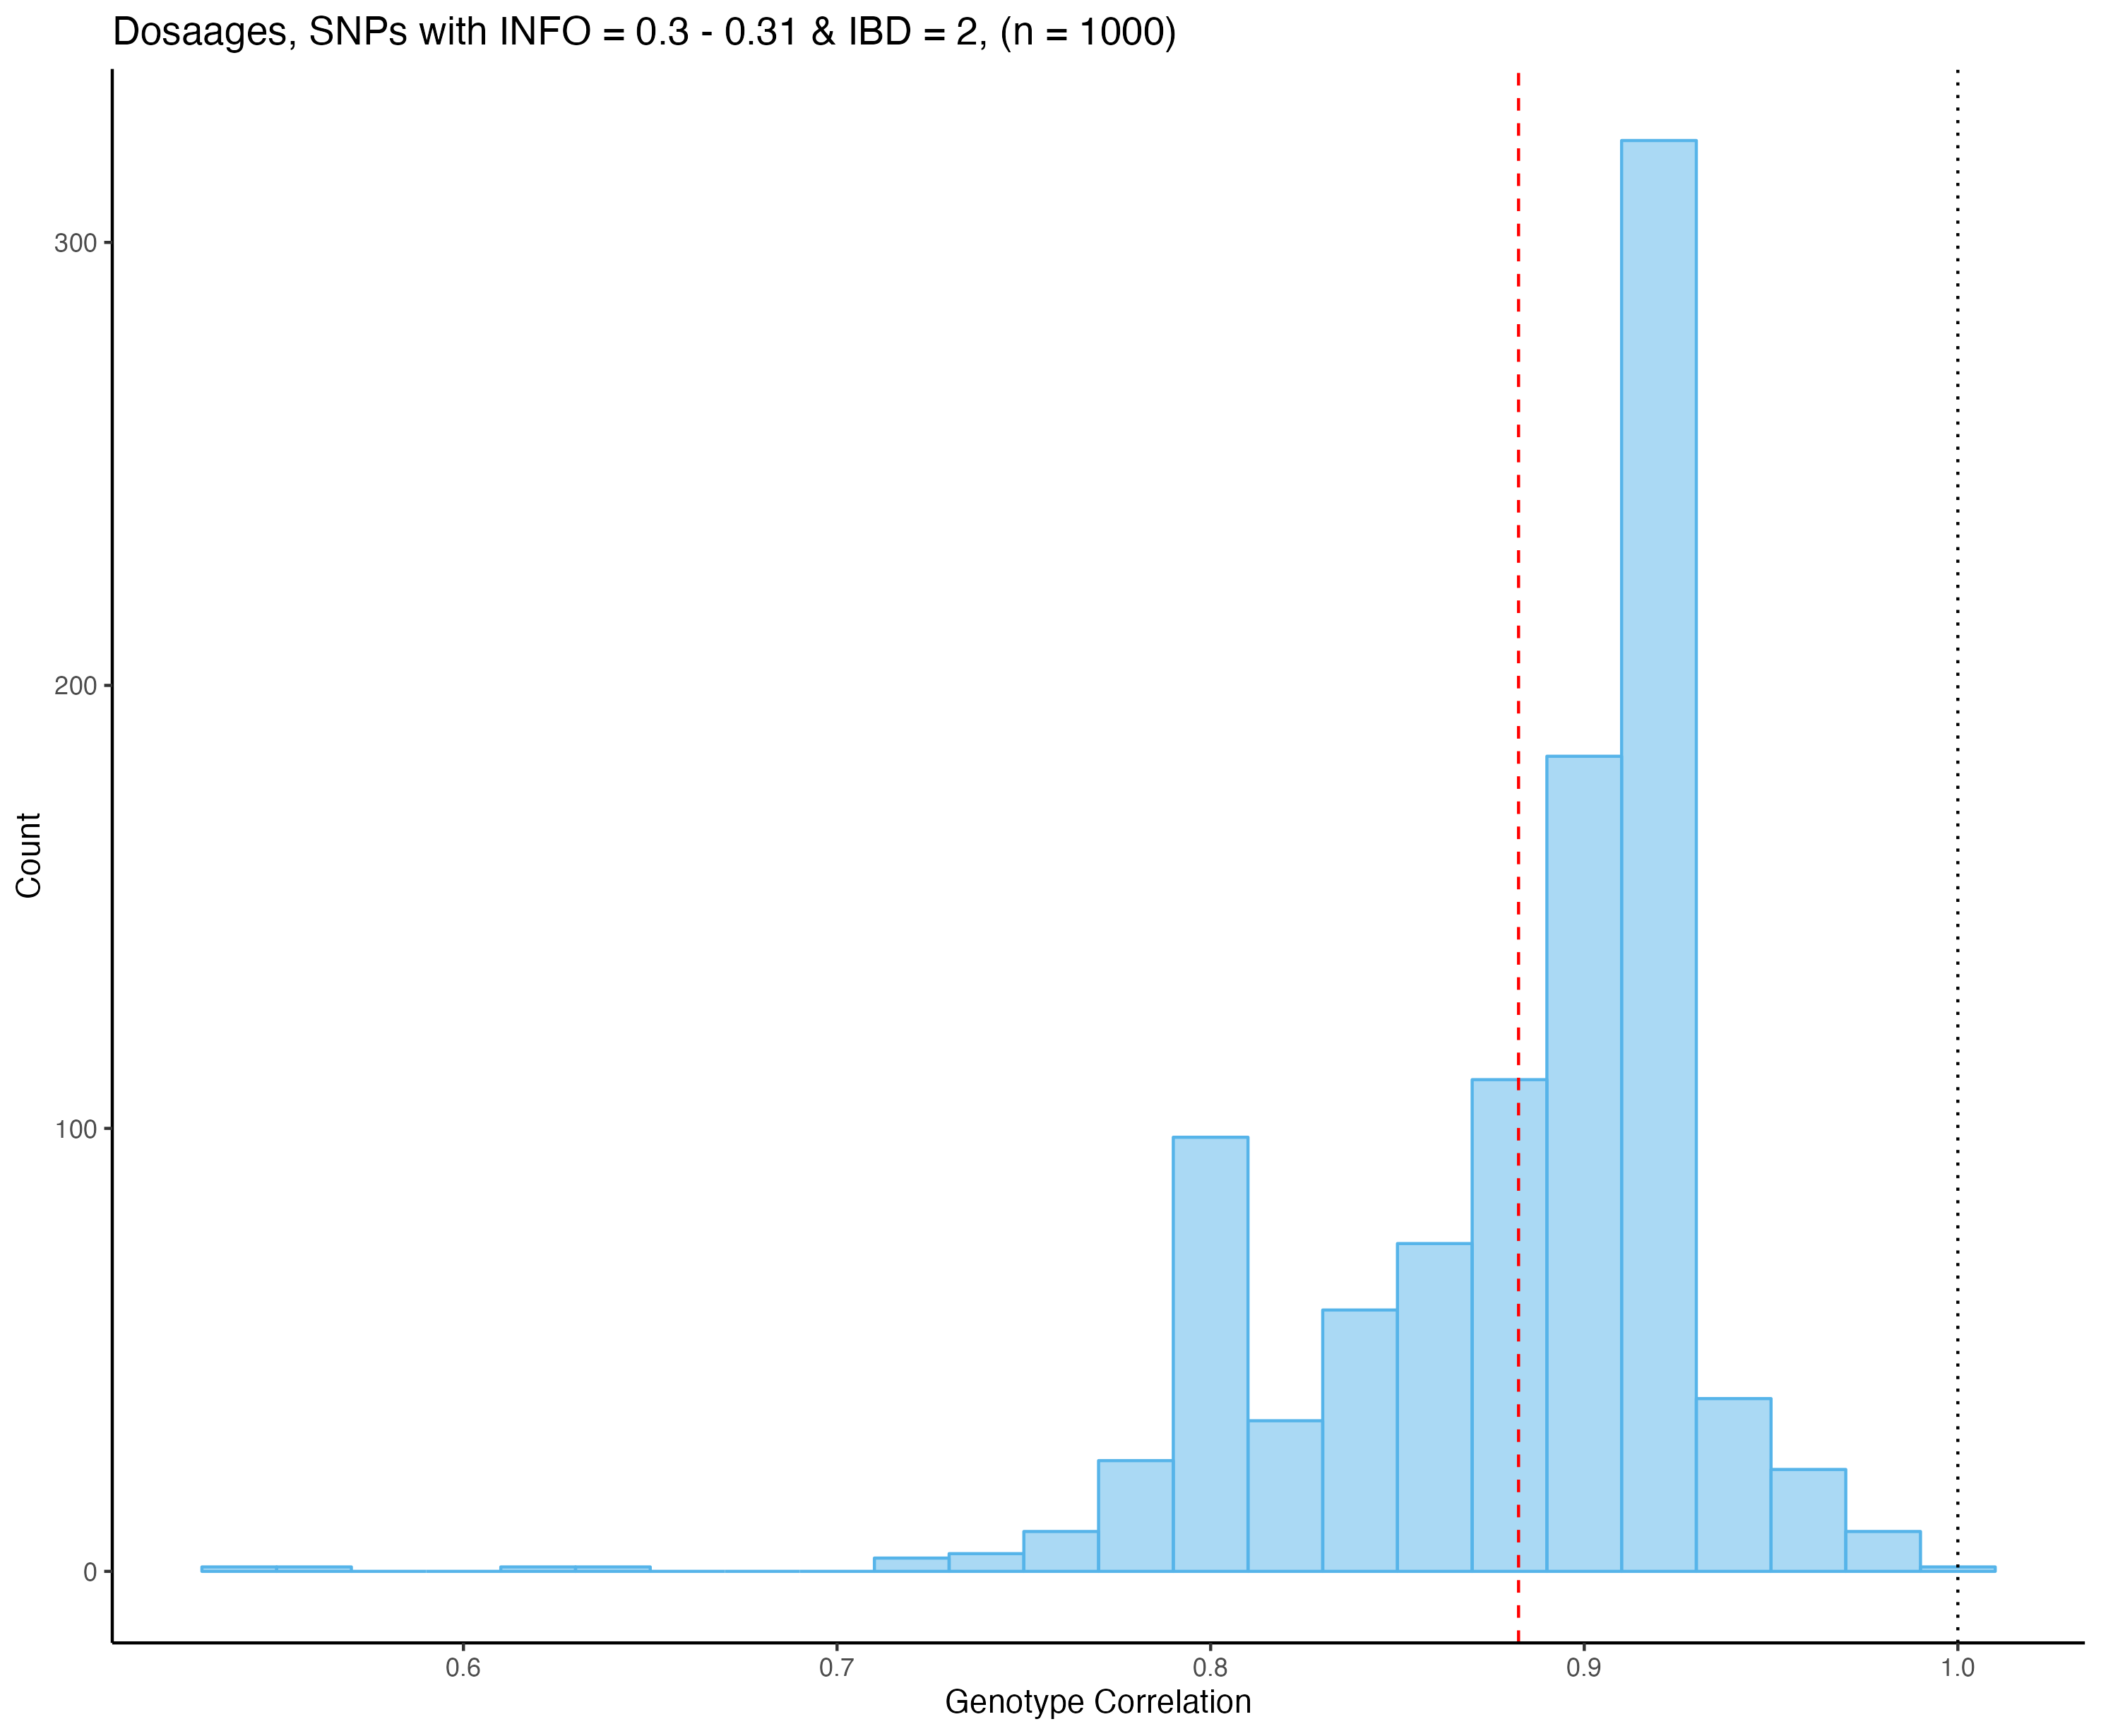
\includegraphics[width= .85\textwidth]{fig/DS-2-i30.png}
      
\end{figure}

\end{frame}



% We would expect to these correlation to be 0 but as 
% the info score decreseas below zero the correlation deviates more from zero. 
% unlike overall trend here the situation is worse for dosages than hard-calls

\begin{frame}{Mean Genotypes (info score)}{IBD = 0}

      \begin{figure}

            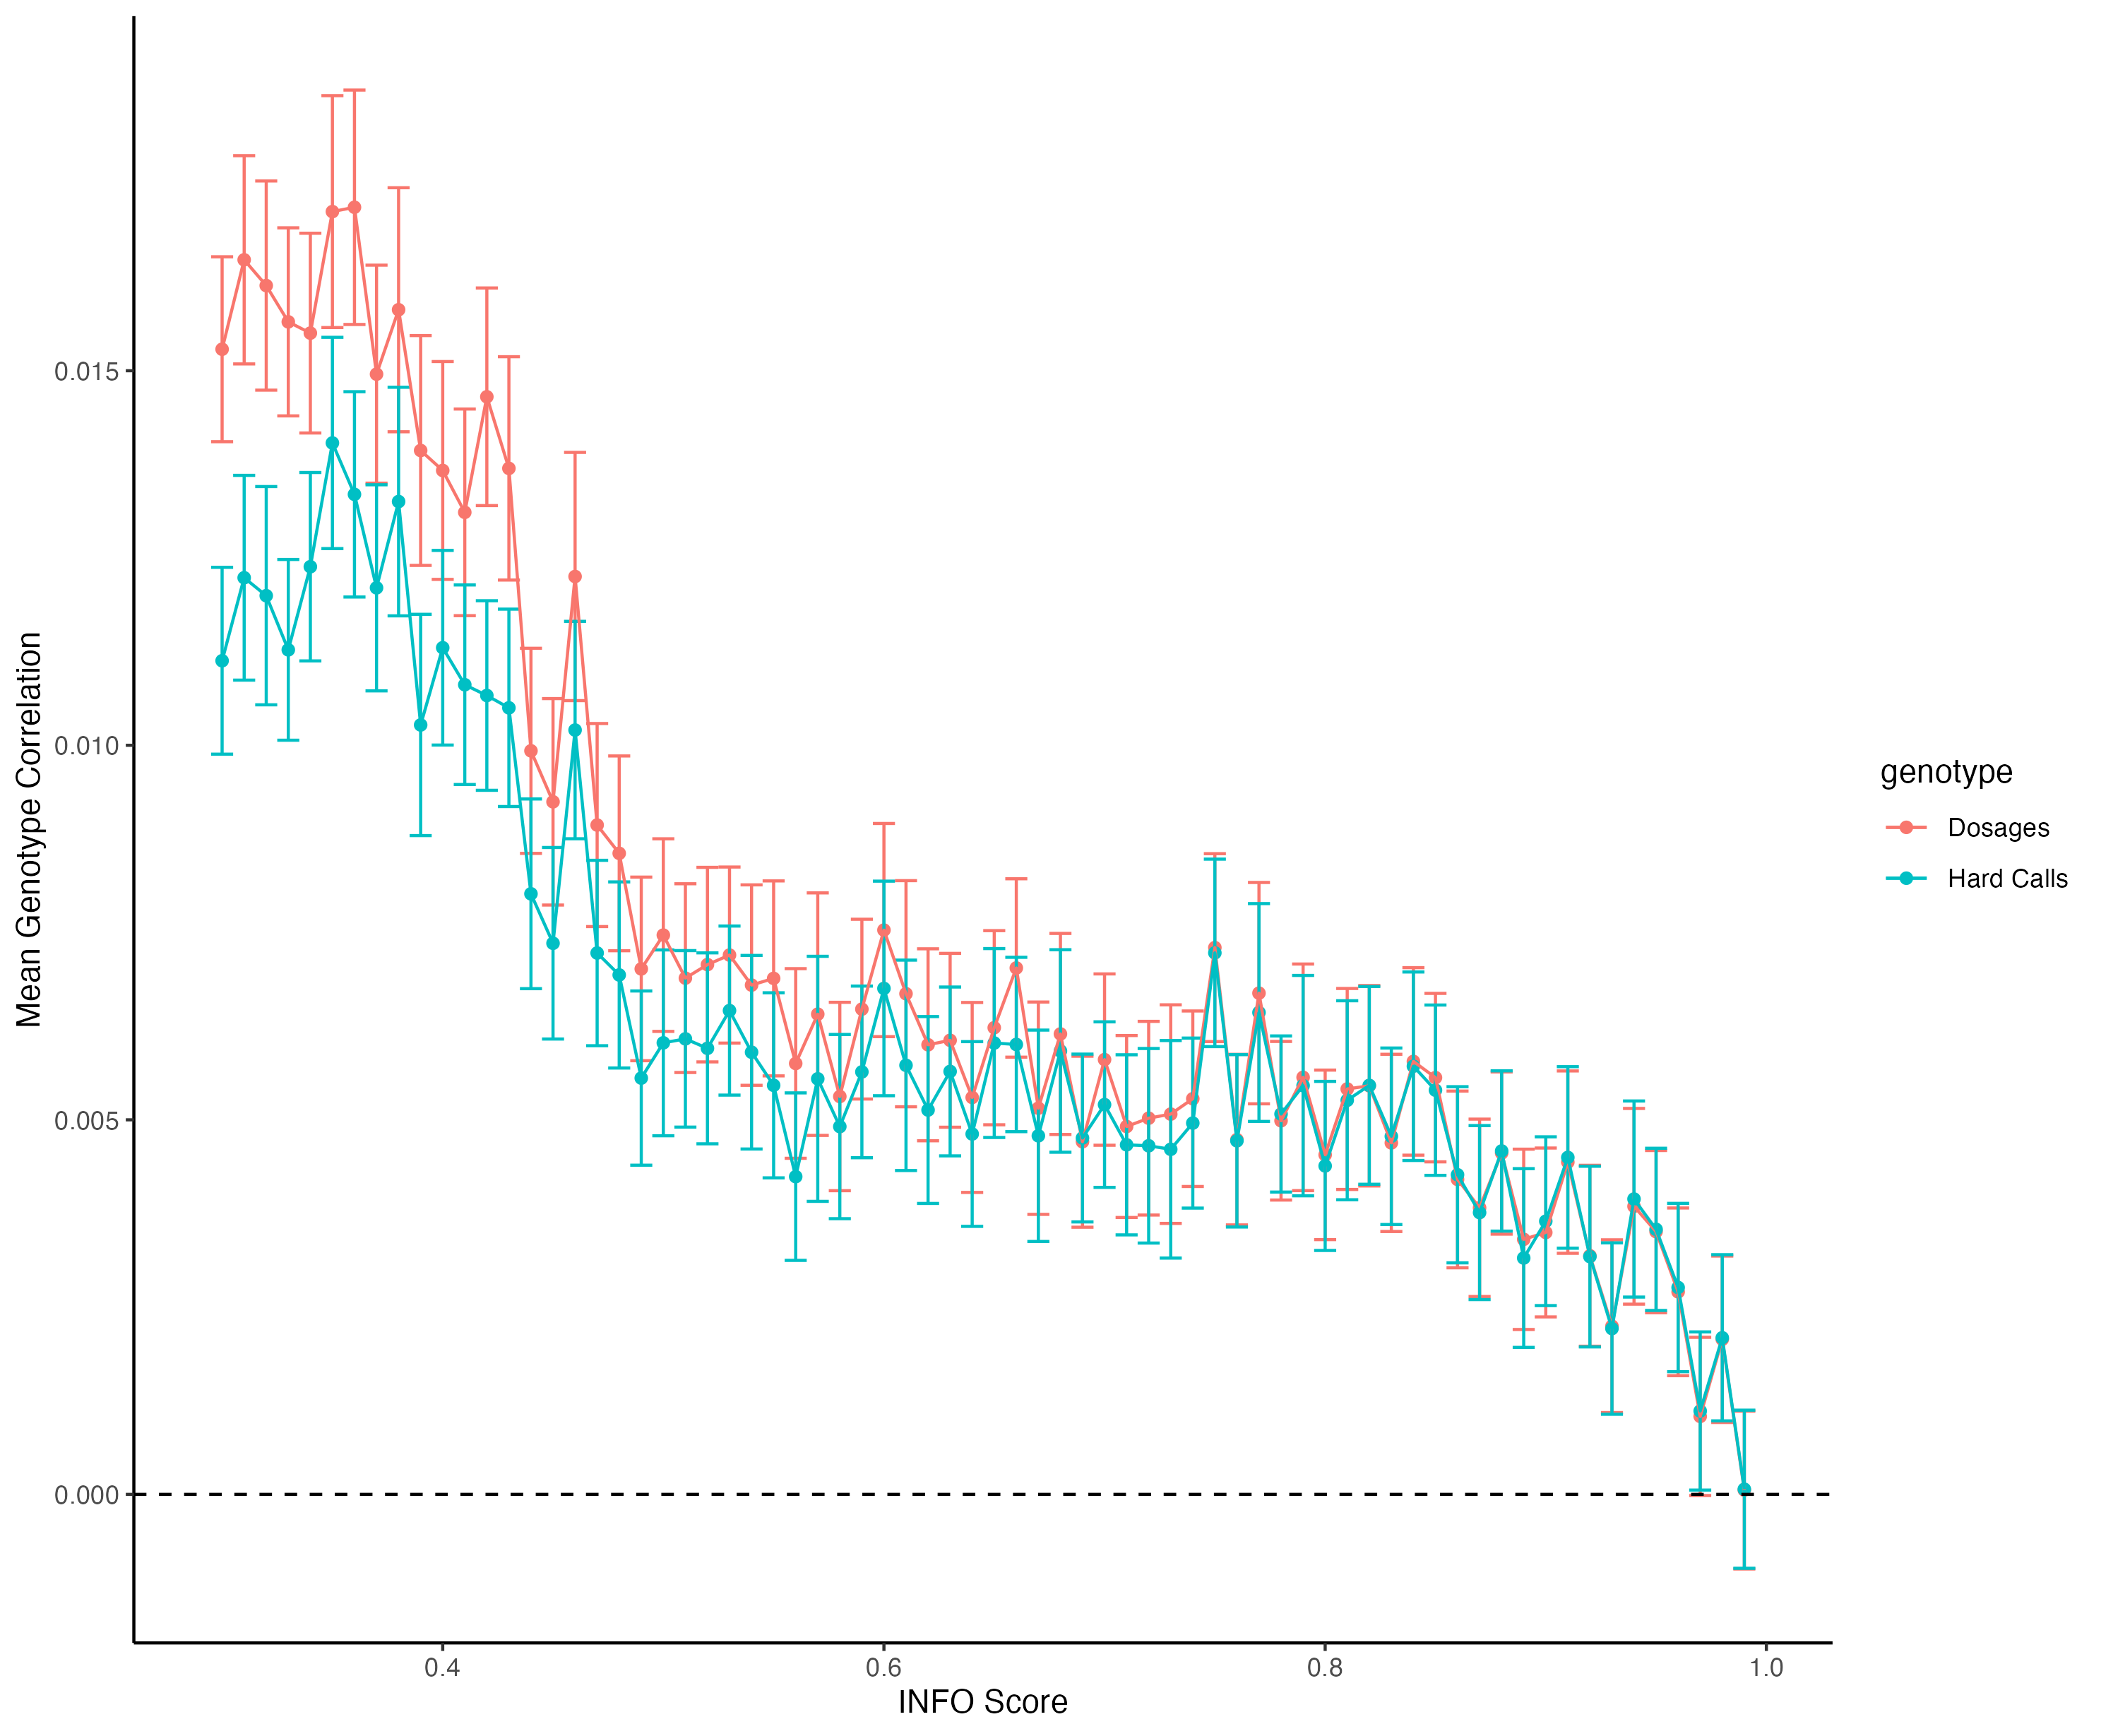
\includegraphics[width= .85\textwidth]{fig/mean_gt_by_ibd_0.png}
            
      \end{figure}

\end{frame}



\begin{frame}{Mean Genotypes (info score)}{IBD = 1}

      \begin{figure}

            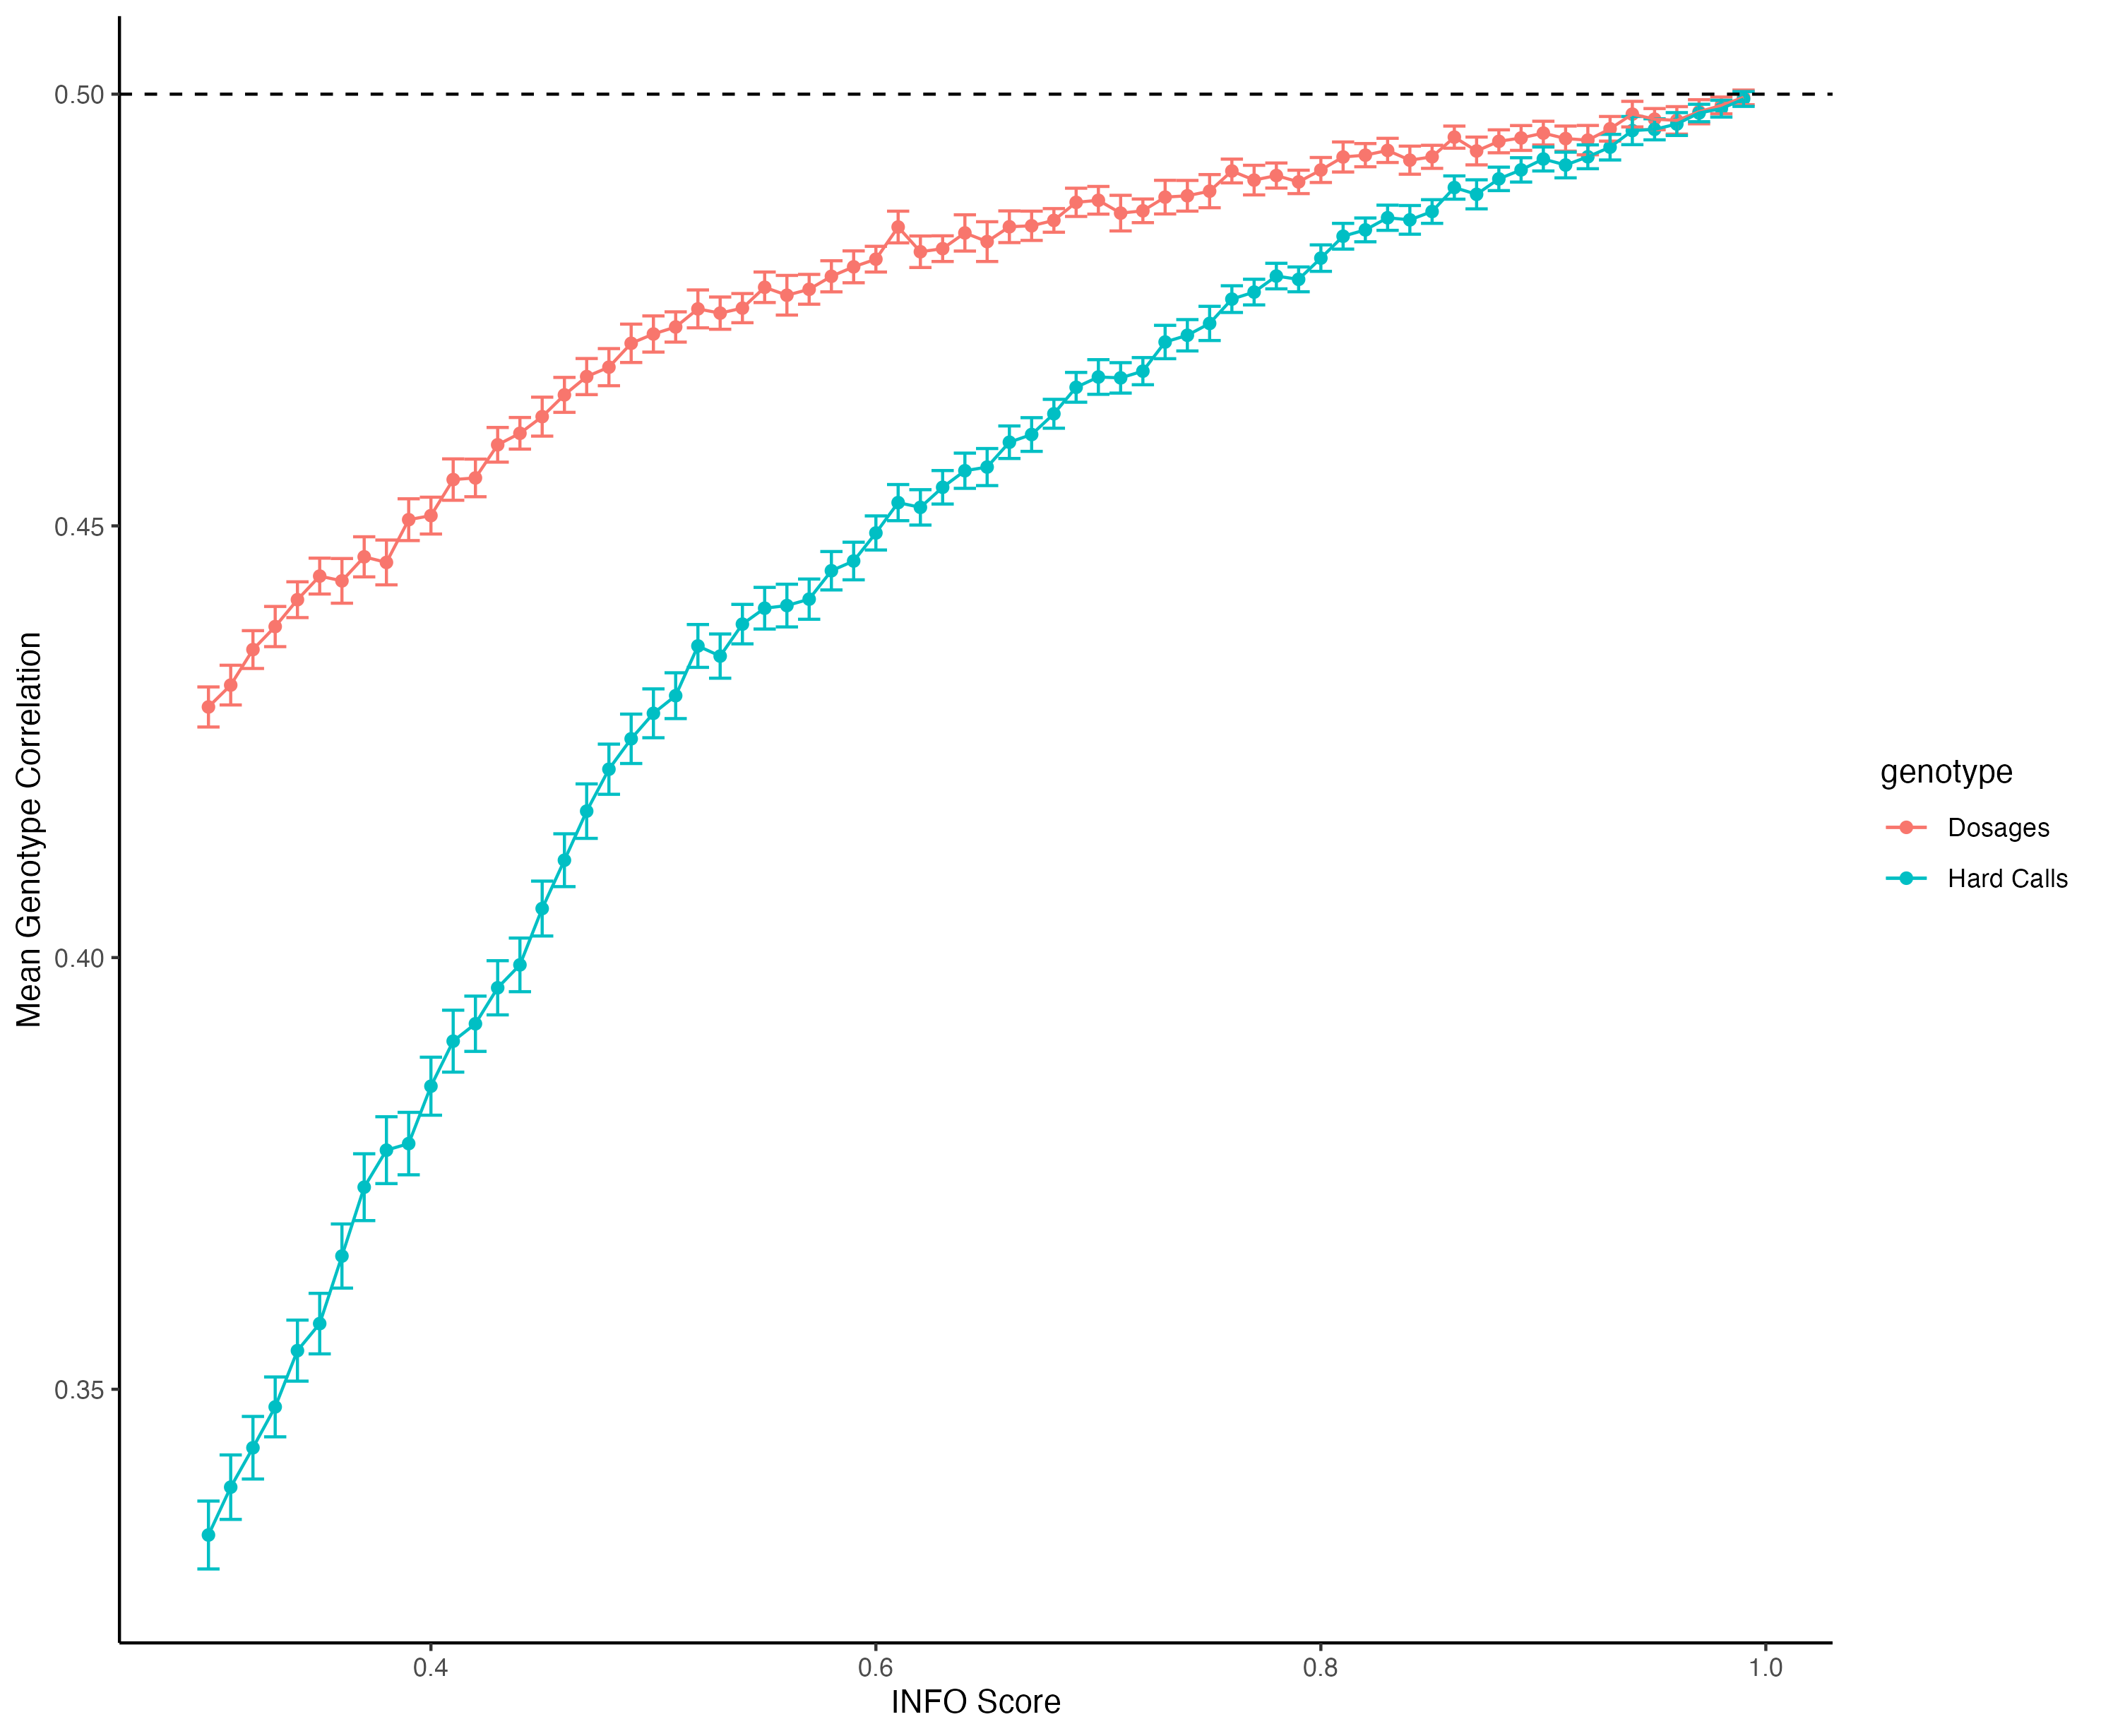
\includegraphics[width= .85\textwidth]{fig/mean_gt_by_ibd_1.png}
            
      \end{figure}

\end{frame}


% ibd 2 is not used in sib-gwas because we are using genotype differences between siblings so 
% IBD should not contribute because they are identical and there is no difference, 
% but here we are showing is that that IBD2 state is not identical between pairs for quality SNPs
% when we are using low quality SNPs. The situation here is worse for hard calls.
% so becuase they are not identical these IBD2 is going to contribute to Sib-Gwas estimate and it shouldn't be
% it shouldn't contribute at all 


\begin{frame}{Mean Genotypes (info score)}{IBD = 2}

      \begin{figure}

            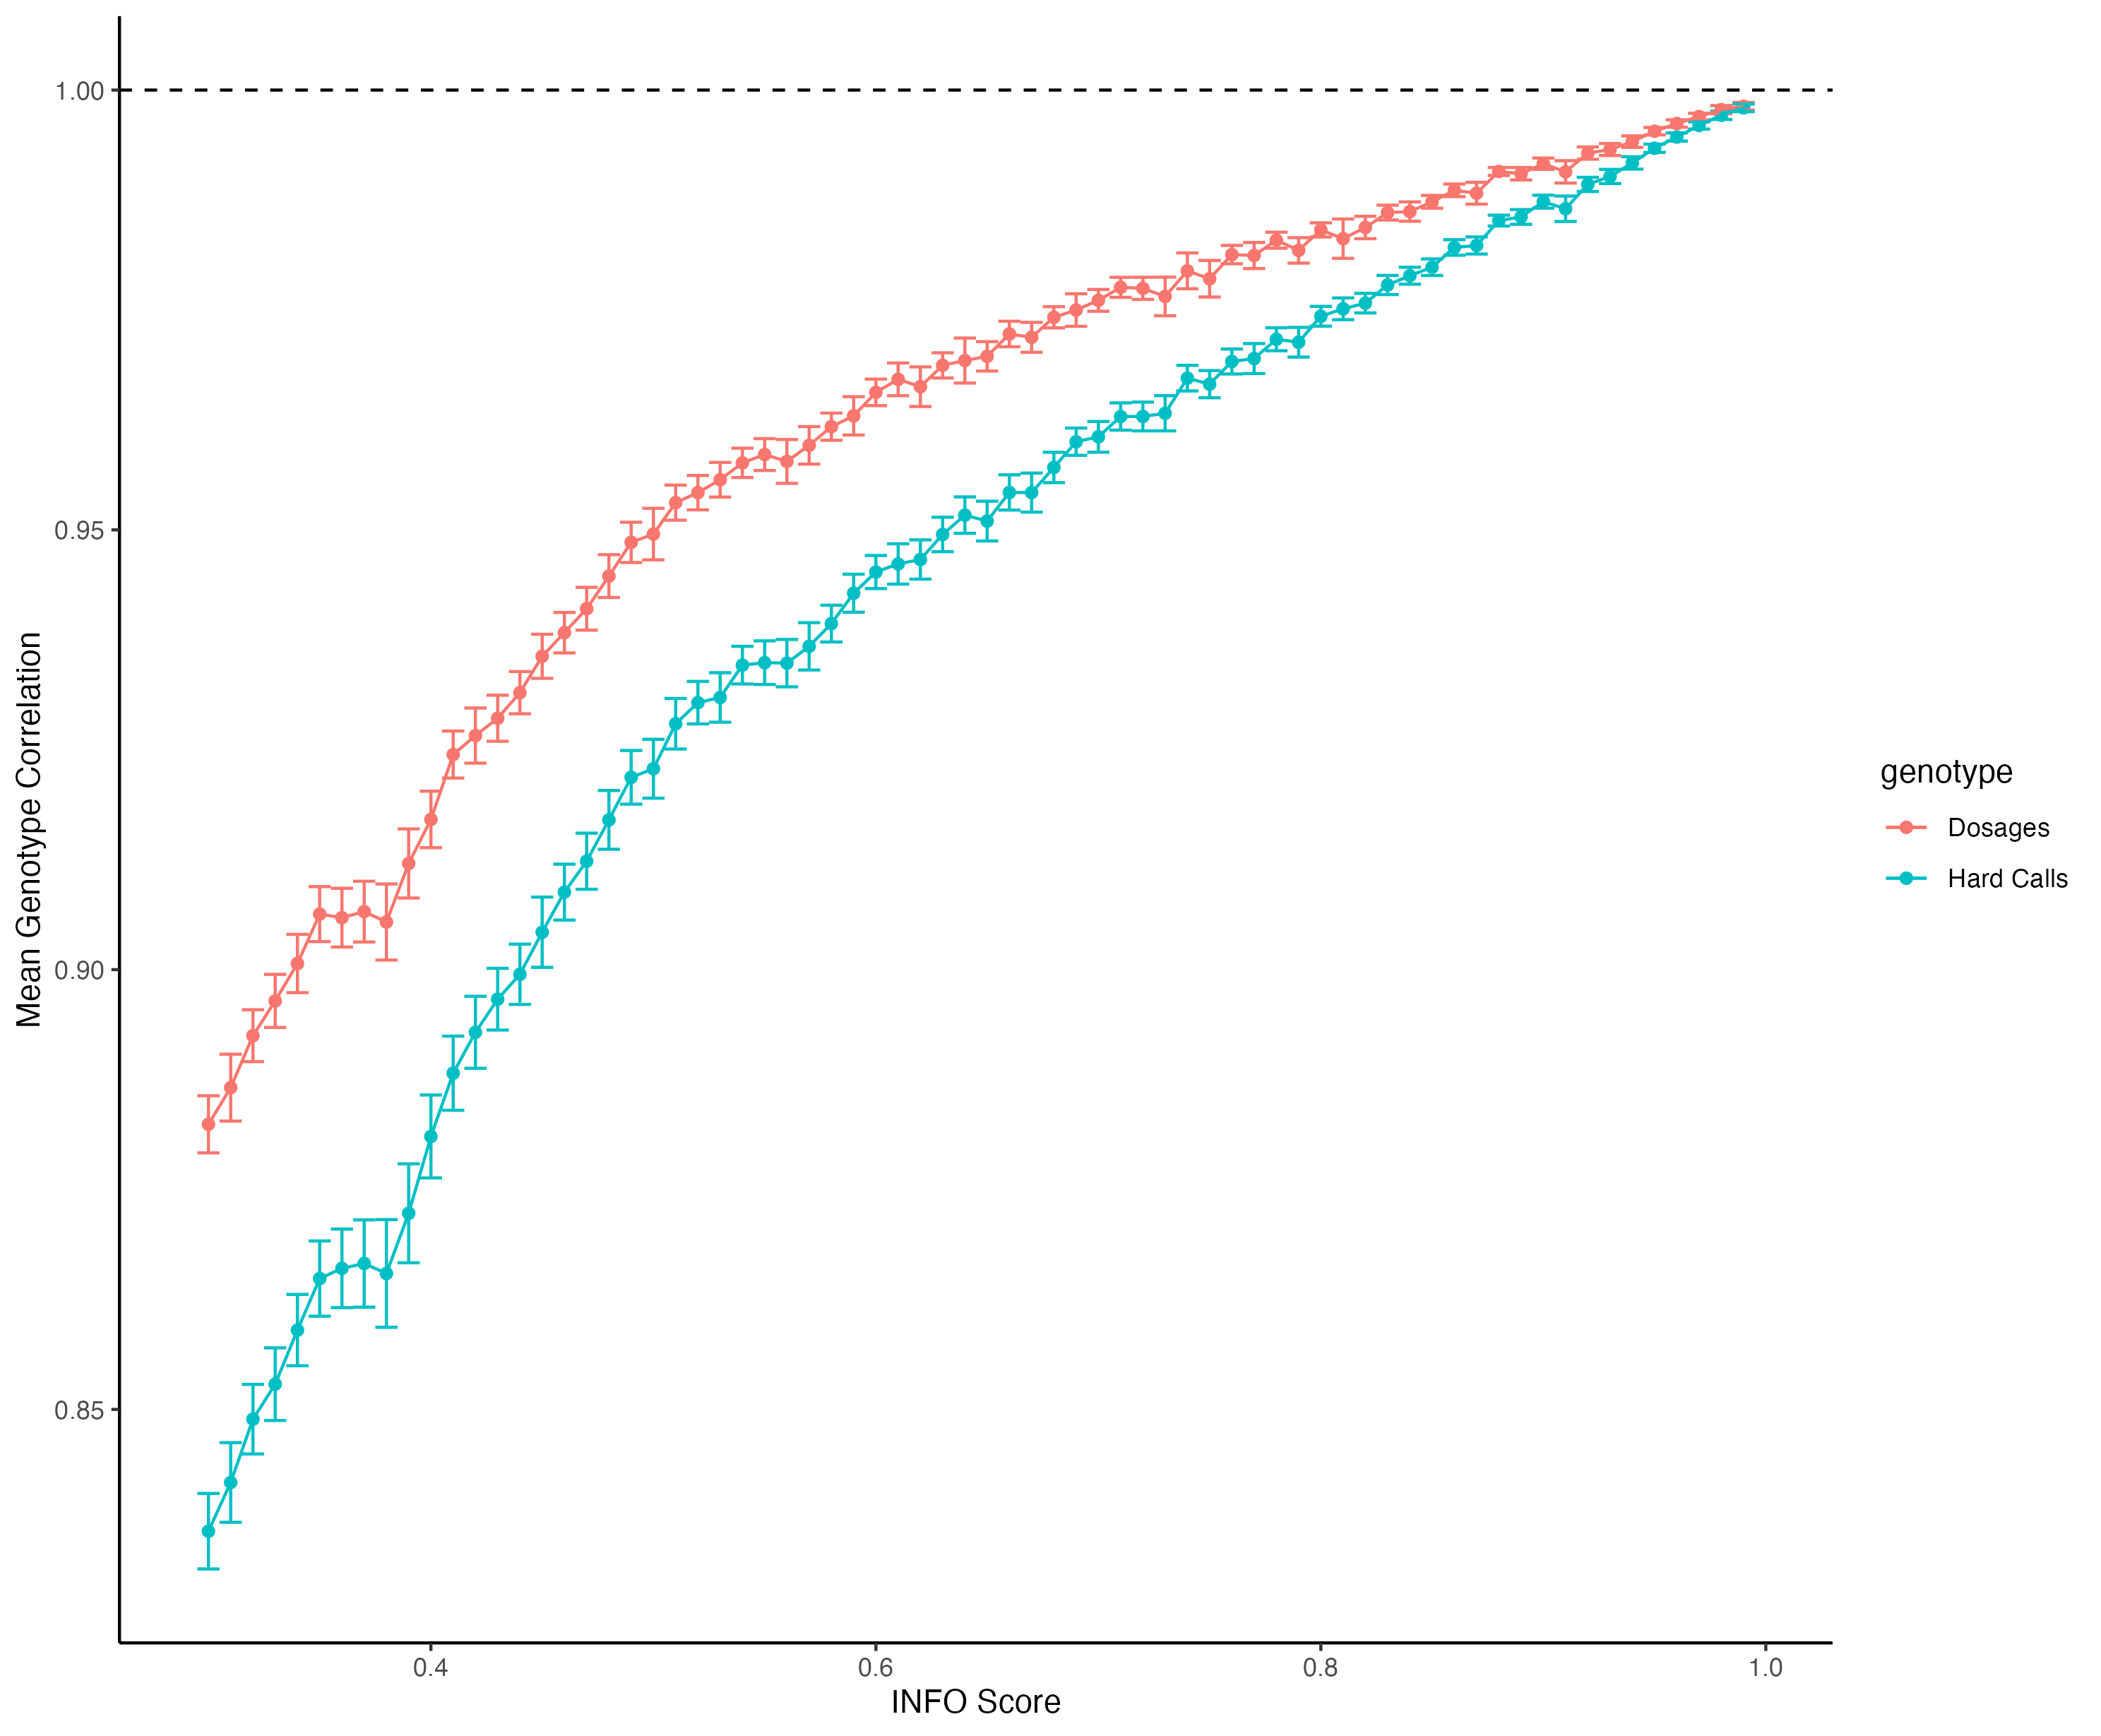
\includegraphics[width= .85\textwidth]{fig/mean_gt_by_ibd_2.png}
            
      \end{figure}

\end{frame}




\begin{frame}{Mean Genotypes (info score)}

      \begin{figure}

            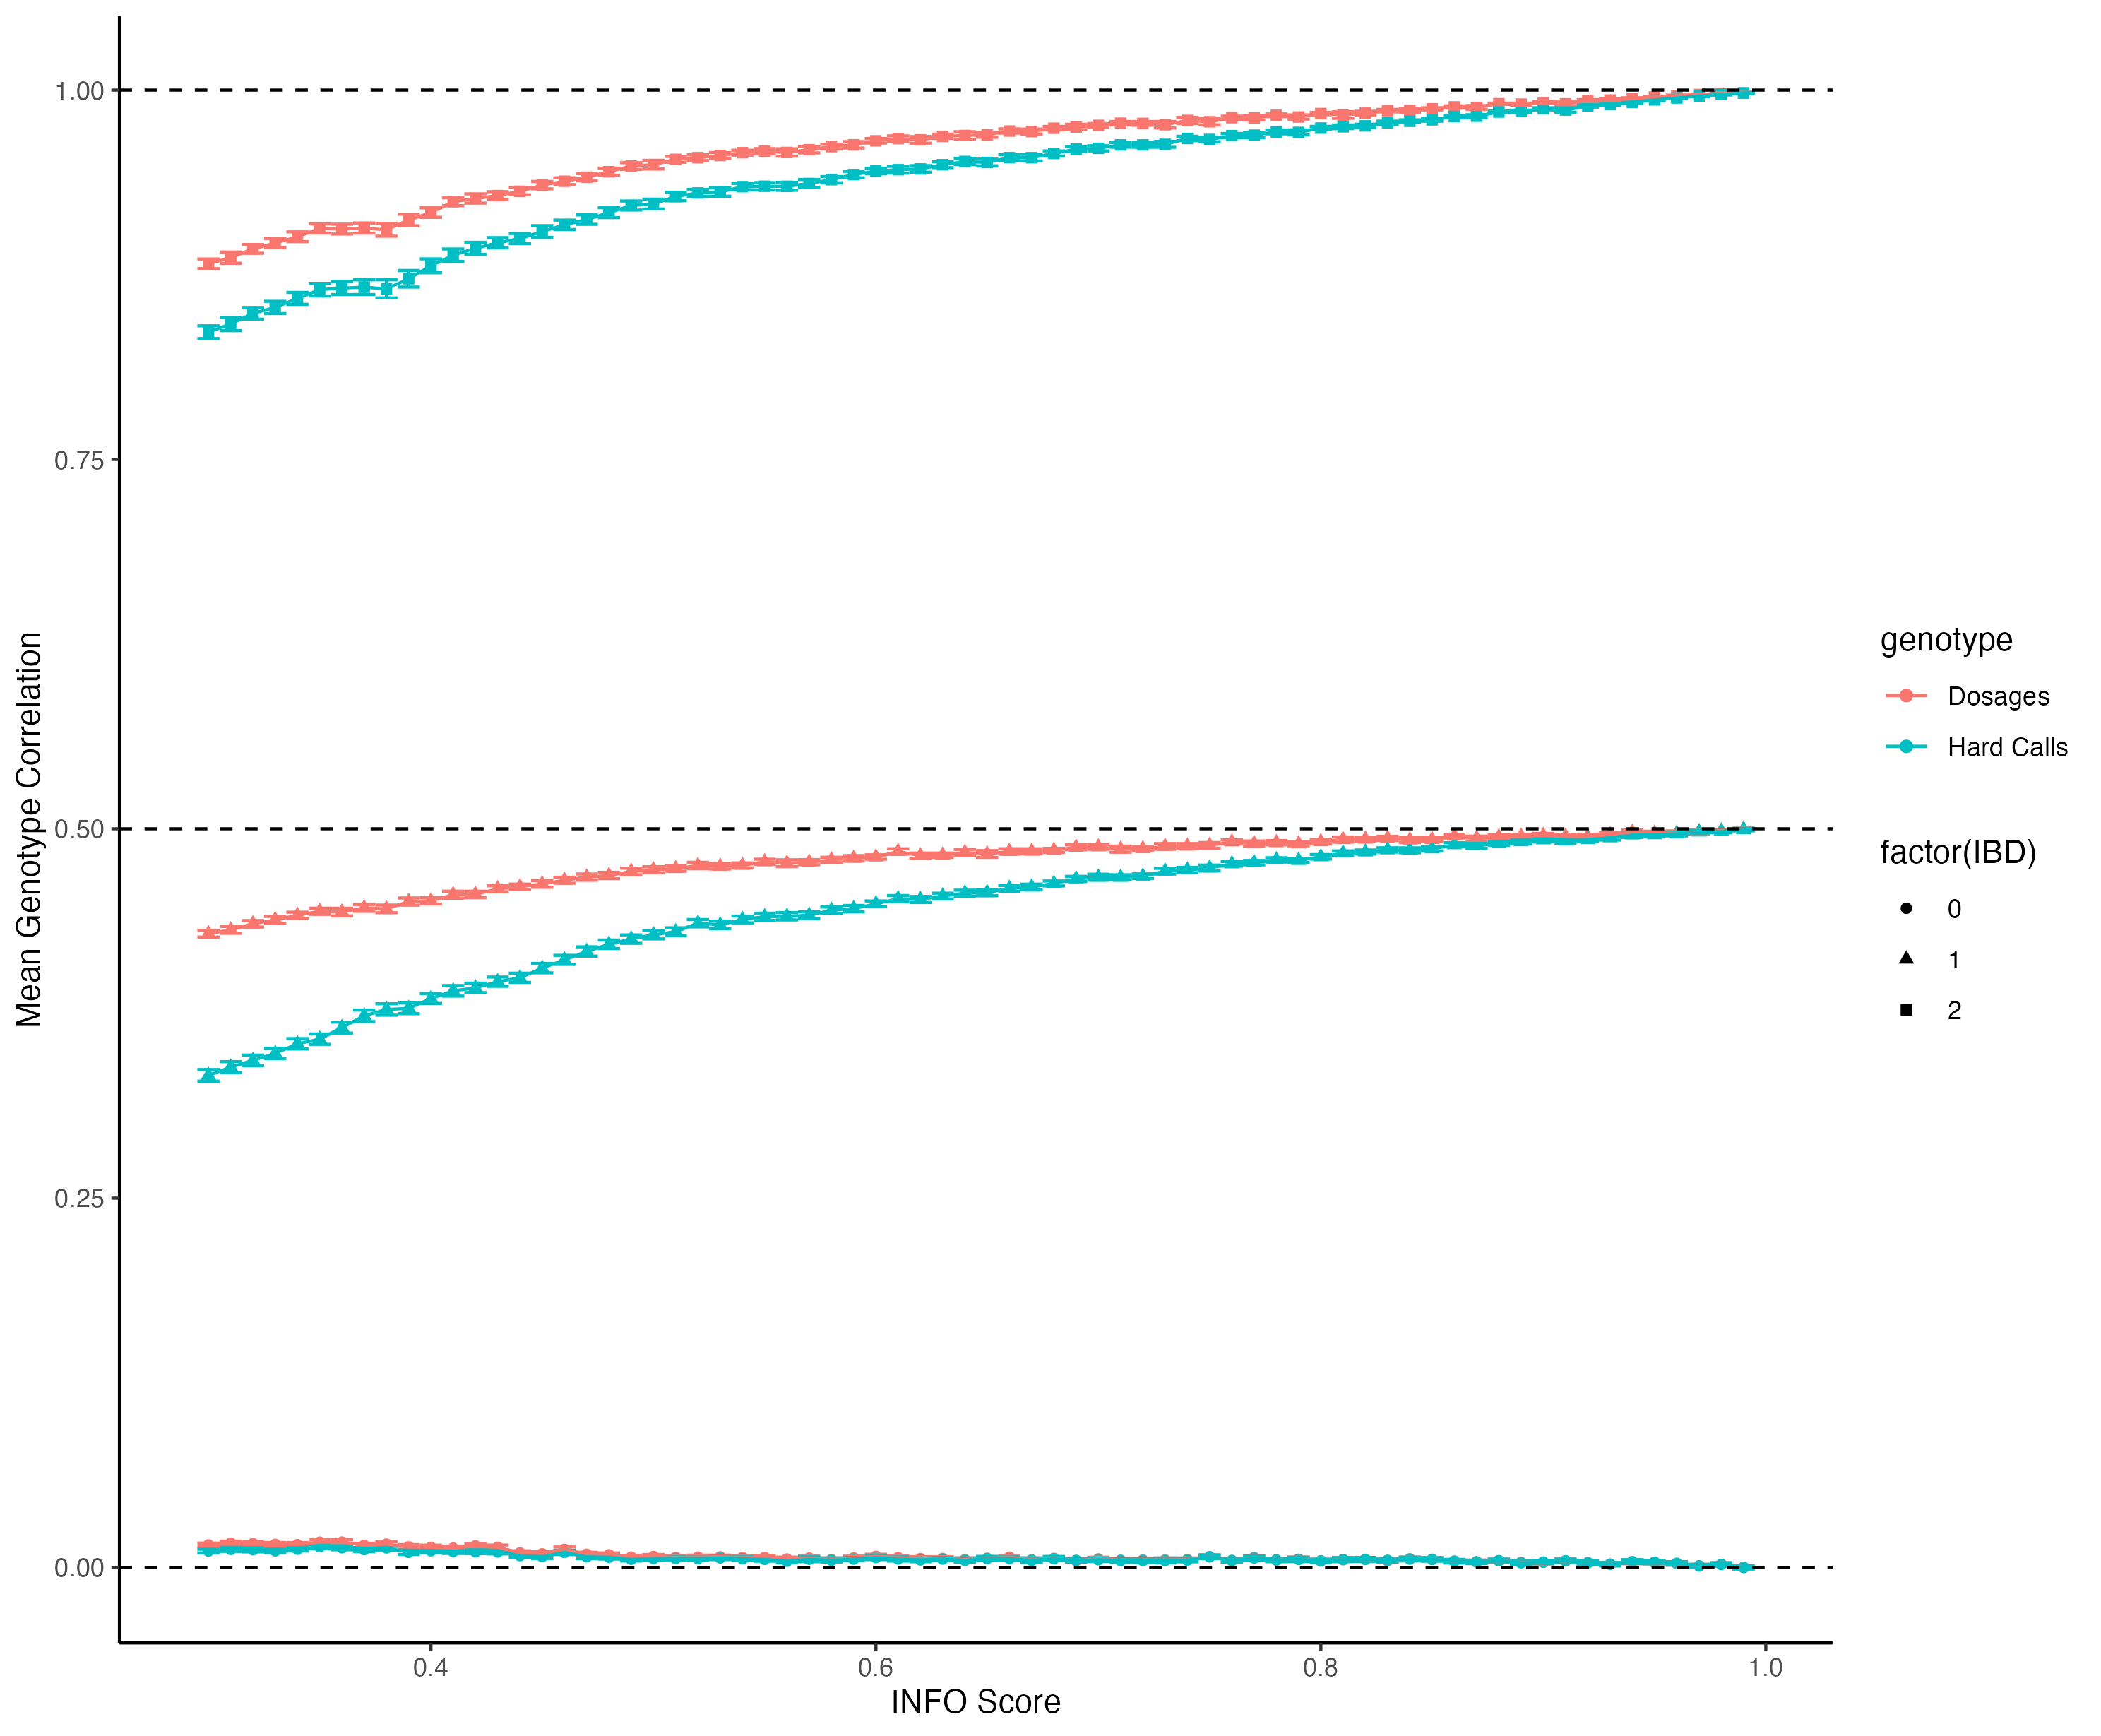
\includegraphics[width= .85\textwidth]{fig/mean_gt_by_ibd.png}
            
      \end{figure}

\end{frame}





\section{WGS Data \& UKB RAP}



\begin{frame}{Why We Need WGS Data?}
      

      \begin{itemize}
            \item We showed that imputed data doesn't have the expcted properties for the family based analysis.
            because the correlation deviates from the theoretical expectations. % and this is ture for both parent-offspring
            % and sibling pairs for both dosages and hard-calls data
            \item What we are concerned and don't understand is that what is the downstream consequences of this problem is for 
            family based GWAS.
            \item Ideally, we would compare the imputed genotypes with true genotypes so we can get some idea what are 
            the downstream consequences might be on Sib-GWAS. 
            % so we are going to use the whole genome sequencing data in the UKB and comparing that to the IMPUTED data
      \end{itemize}


\end{frame}



\begin{frame}{WGS Data}

      \begin{itemize}
            \item UKB has released whole genome sequencing (WGS) data
            on 30th November 2023 from half a million volunteers.
            \item First they released 200K version in 2021.
      \end{itemize}

      \begin{figure}
            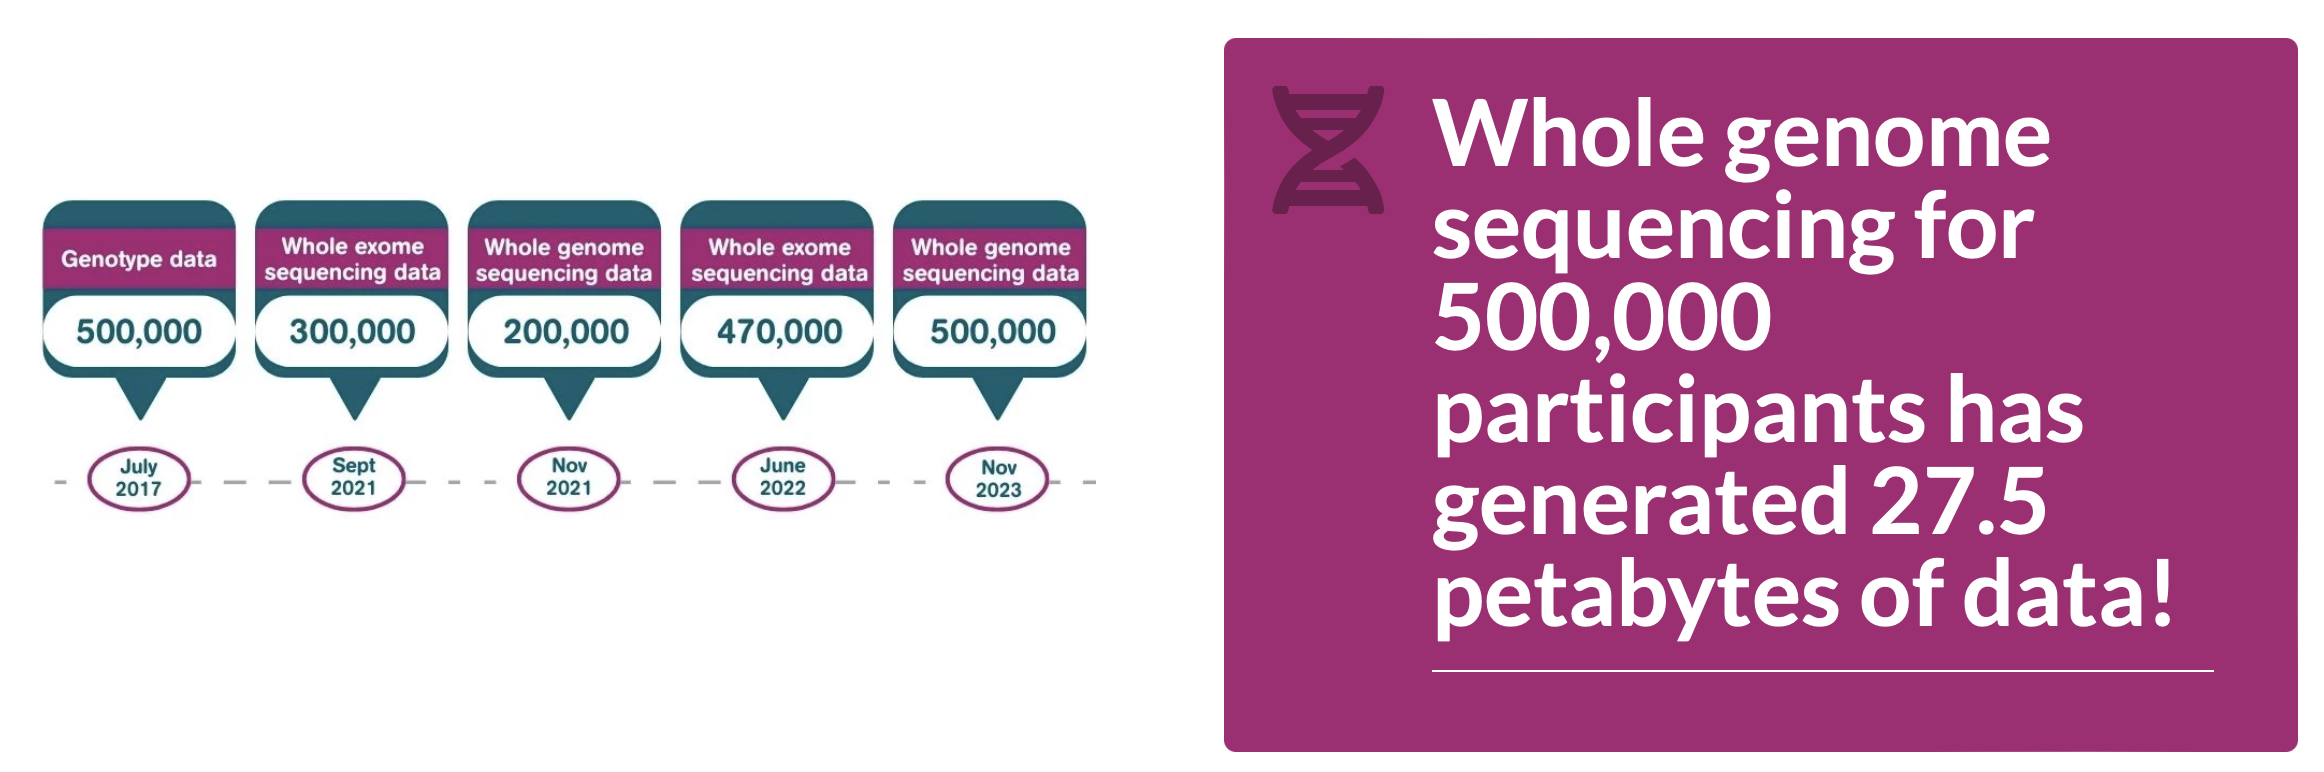
\includegraphics[width = \textwidth]{fig/sc1.png}
      \end{figure}
      

\end{frame}



\begin{frame}{UKB-RAP Setup}

      \begin{itemize}
            \item First you create an account get approved on UKB-AMS.
            % which is the access management system of the ukb
            \item Then you should be added as a part of SSGAC on the platform.
            % I don't remeber how exactly I did this step but I think Chelsea
            % added me to the group on SSGAC
            \item Then using your account you can access the RAP-Platfrom.
            \item On the RAP platform you have access to different tools
            like Jupyterlab \& R studio. 
            % \item You can access to a terminal inside the Jupyterlab.
            % But nothing is installed on it you have to install it yourself.
            \item You should first create a project then you can access tools \& data.
            \item Upon project creation you should provide your application ID to access the data.
      \end{itemize}

      
\end{frame}



\begin{frame}{How to access WGS Data}

      \begin{itemize}
            \item Getting an application ID is a separate process in which you
            should apply to get access to the data and you should specify which
            data and for what purpose you want to use. It takes some days to get
            approved.
            \item But fortunately you don't need to do this.
            \item Get the application ID from Chelsea. If you are already 
            a member of the SSGAC on the RAP you can use the application ID on your
            personal profile to get access to WGS data.
            \item You provide the application ID and you should select data bundles you need.
            \item Tabular data and bulk data files
            \item \textit{Addtionall bulk data} files for individula level data later. It takes about 1 or 2 days to dispense data to your project.
      \end{itemize}

\end{frame}


\begin{frame}{Some Important Things}

      \begin{itemize}
            \item Billing: You can used the the \pounds 40 first then you should transfer billing to SSGAC. 
            \item WGS Individual level data is in this path:
            \\yourproject:/Bulk/DRAGEN WGS/Whole genome variant call files (VCFs) (DRAGEN) [500k release]
            \item Will PLINK or BGEN versions be released?
            \\ PLINK 2.0 and BGEN versions for both the DRAGEN and GraphTyper joint variant calls are planned to
            be released in 2024.
      \end{itemize}

\end{frame}


\begin{frame}{Some Important Things (cont'd)}

      \begin{itemize}
            \item Use TABIX for now with VCF Files. It is much faster than plink2 for VCF files when
            it is used with .tbi index.
            \item CAUTION: Individual IDs are getting randomized for each application ID.
            You might get results that are compeletly random if you don't know this.
      \end{itemize}

\end{frame}



\begin{frame}{Next Step}

      \begin{itemize}
            \item We are going to estimate a sib-difference regression on the
            real WGS data then we can ask what we would obtain if we instead use
            imputed data.
            \item Then we can assess the bias that comes from using imputed data.
            
      \end{itemize}

\end{frame}


\begin{frame}[plain]

      \huge{Thank You for your Attention!} \\
      % thank you everyone
      % thank you jon for the code review and thank you Alex for your valuable comments and feedbacks in previous days.
      % thank you everyone for your attention.
      \vspace{.5in}
      \Large{Please Provide me with FEEDBACKS!}

\end{frame}


\end{document}